%===============================================================================
% APPENDIX: EXTENDED RESULTS
%===============================================================================

%===============================================================================
\section{Extended Results}
\label{app:extended_results}
%===============================================================================

%===============================================================================
\subsection{Extended Results: Reverse Perturbation Analysis}
\label{app:extended_results:reverse_perturbation}
%===============================================================================
\begin{figure}[ht]
    \centering
    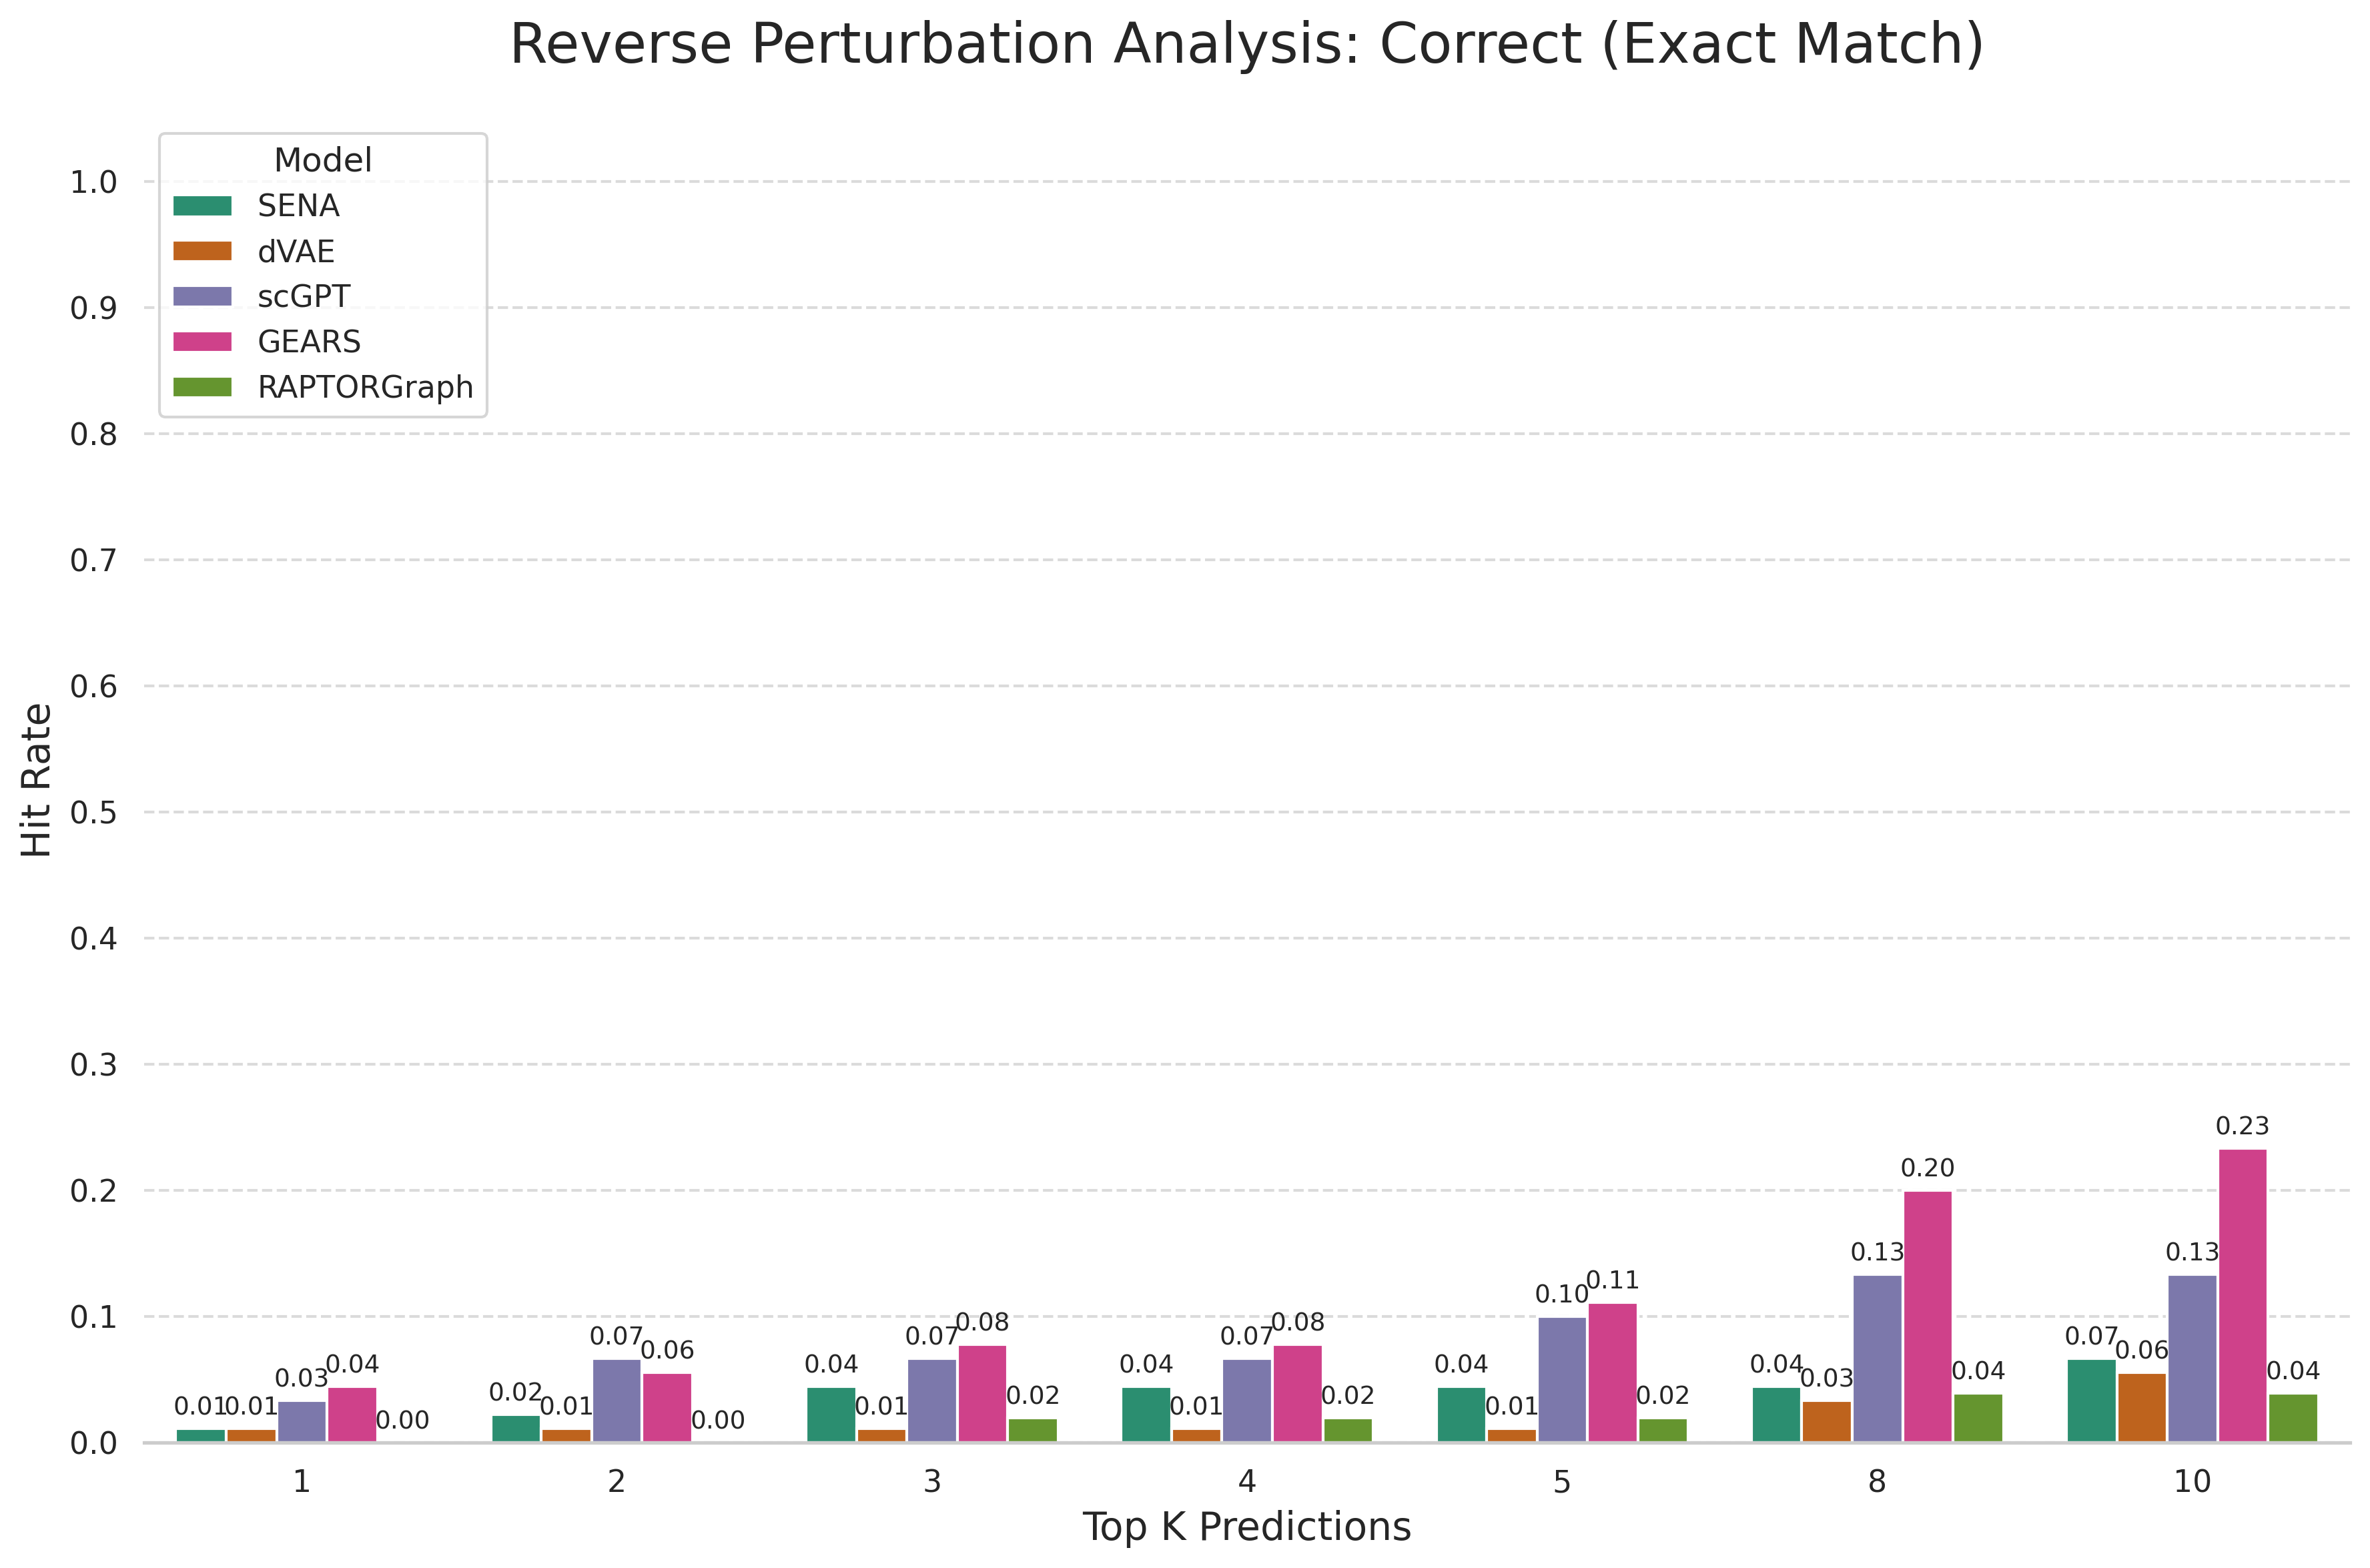
\includegraphics[width=0.75\linewidth]{gfx//results/hit_rate_at_k_correct_exact_match.png}
    \caption{Hit Rate @ K (correct) for the reverse perturbation task.
    The metric queries where the exact true perturbation is correctly identified within the top K ranked predictions.
    Results are averaged over 3 runs.}
    \label{fig:app:hit_rate_exact}
\end{figure}

\newpage

%===============================================================================
\subsection{\revised{Extended Results: Biological Validation of Learned \cmps{}}}
\label{app:extended_results:biological_validation}
%===============================================================================

\begin{figure}[ht]
    \centering
    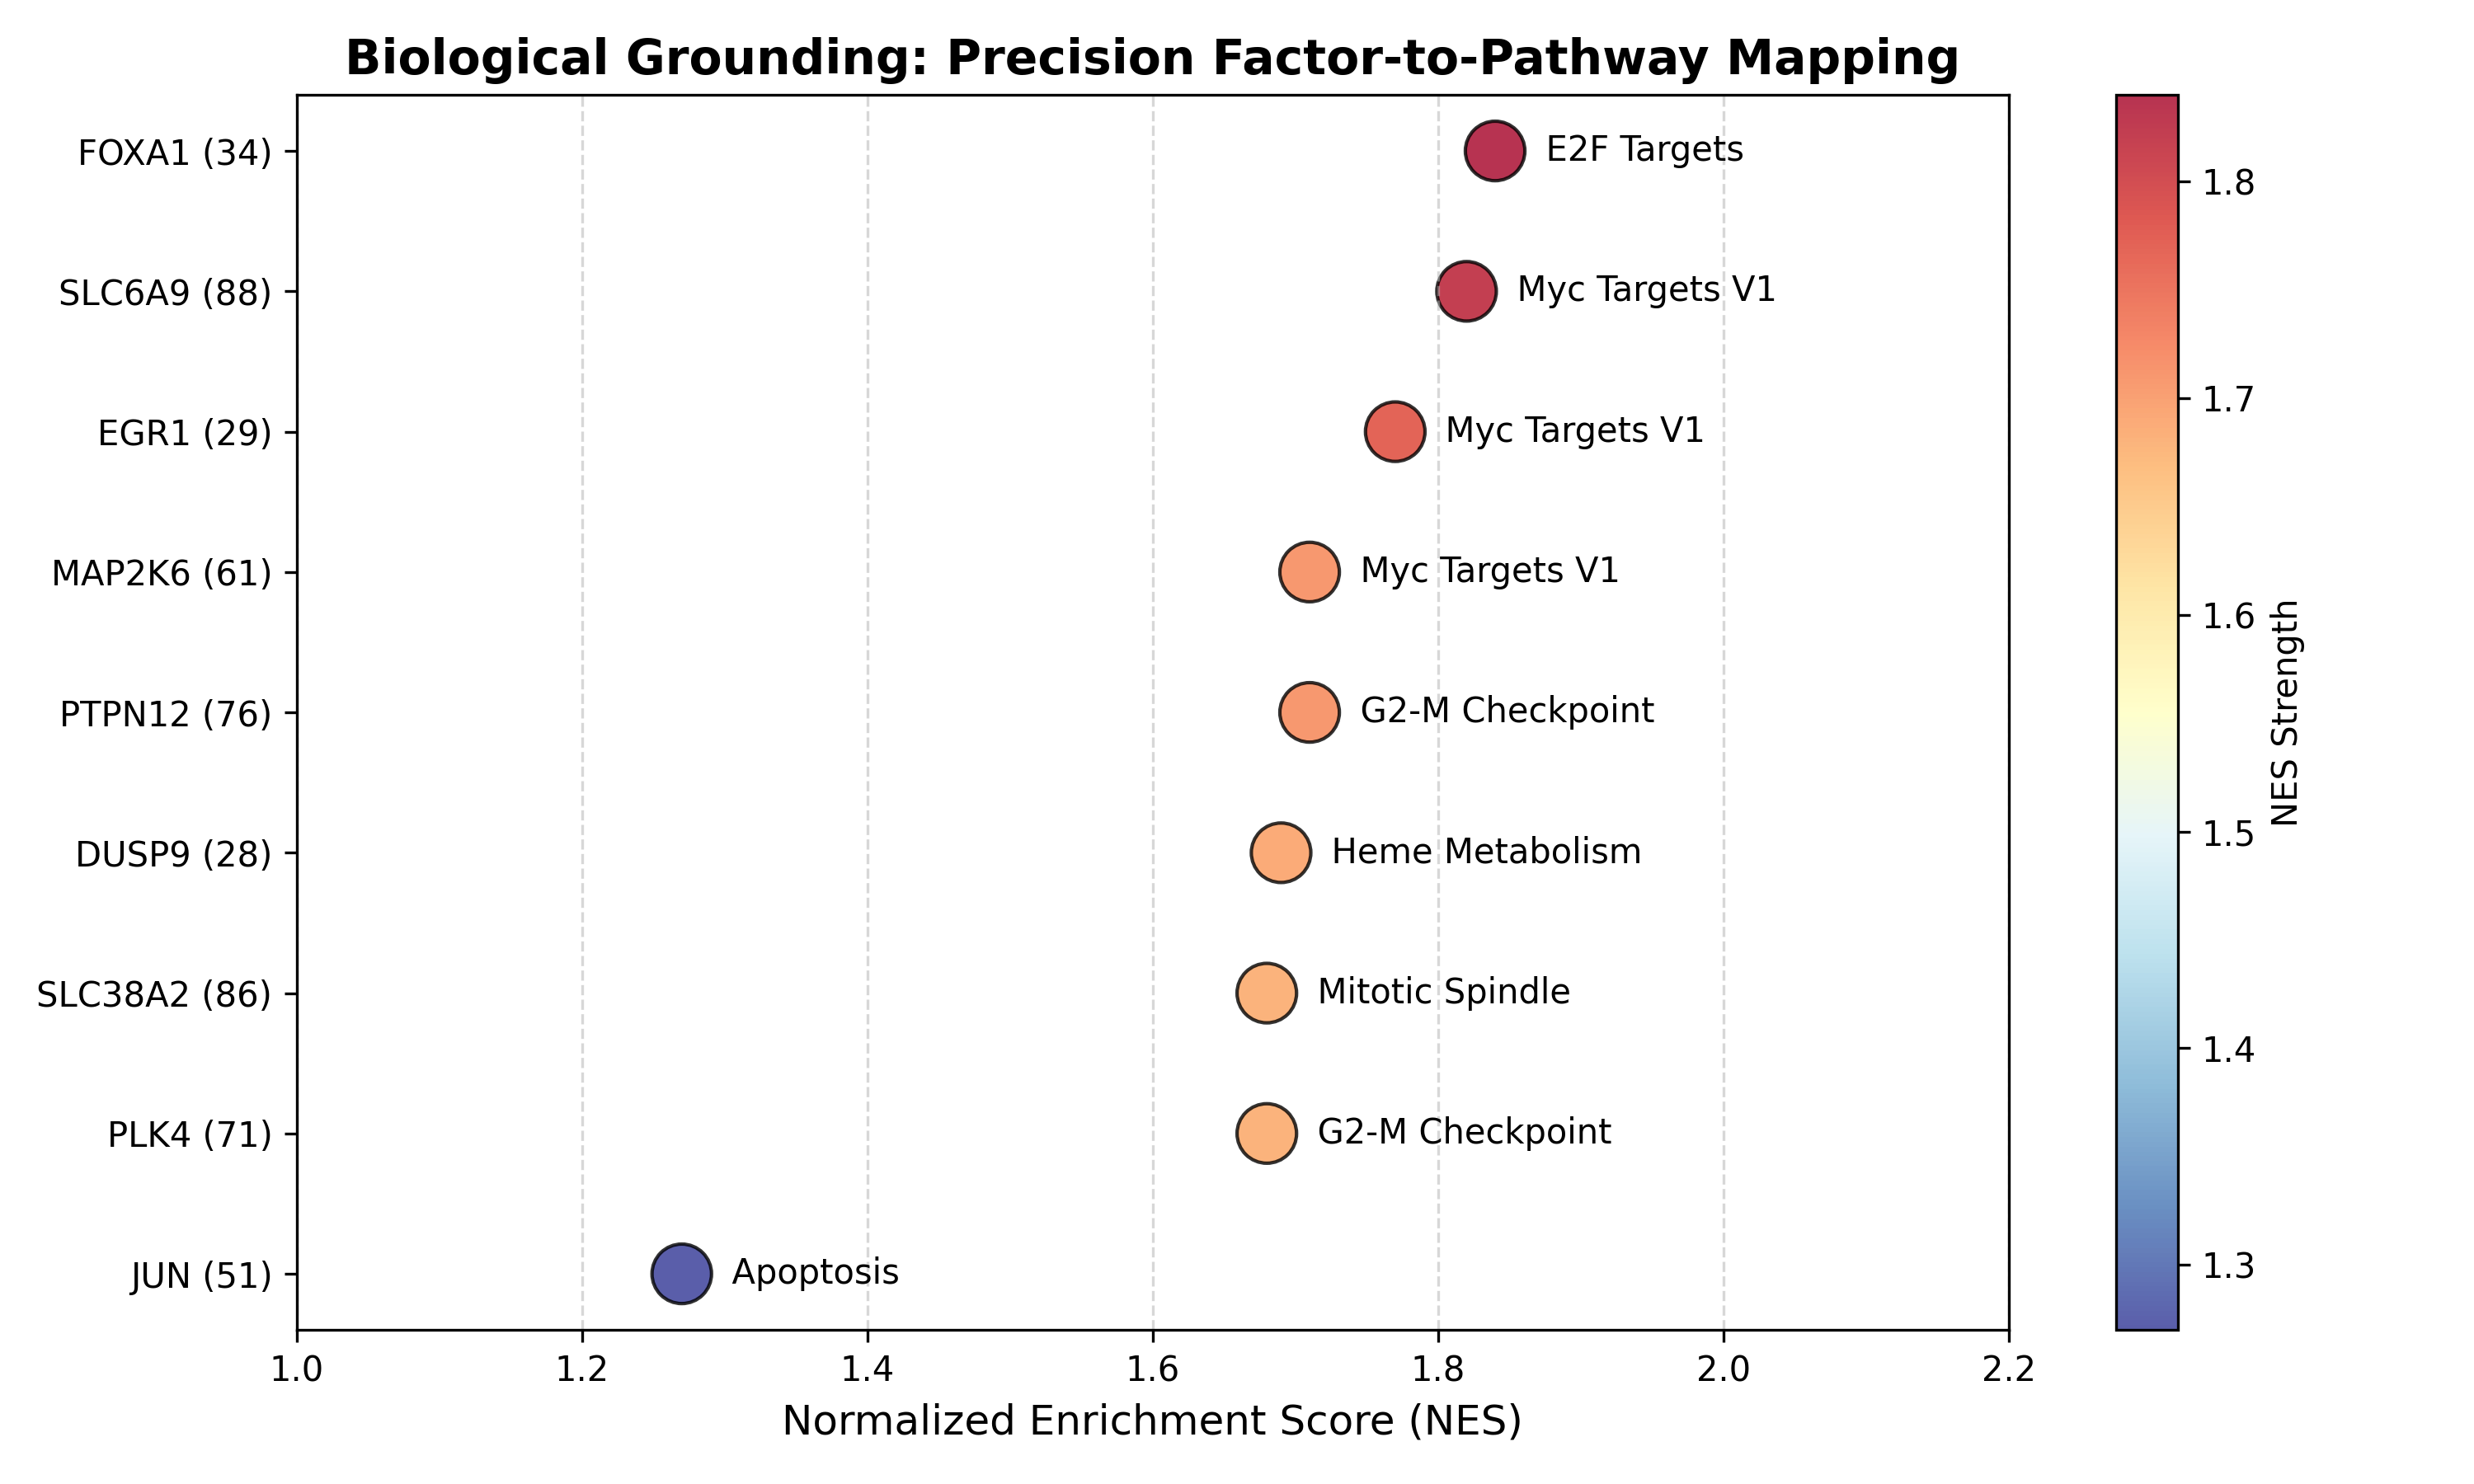
\includegraphics[width=0.8\textwidth]{gfx/rebuttal/fig_gsea_dots.png}
    \caption{\revised{\textbf{Biological Grounding (GSEA Dot Plot).} Visualization of Normalized Enrichment Scores (NES) for top-ranked causal factors, confirming precise mapping to established Hallmark pathways.}}
    \label{fig:rebuttal:gsea_dots}
\end{figure}

\begin{figure}[ht]
    \centering
    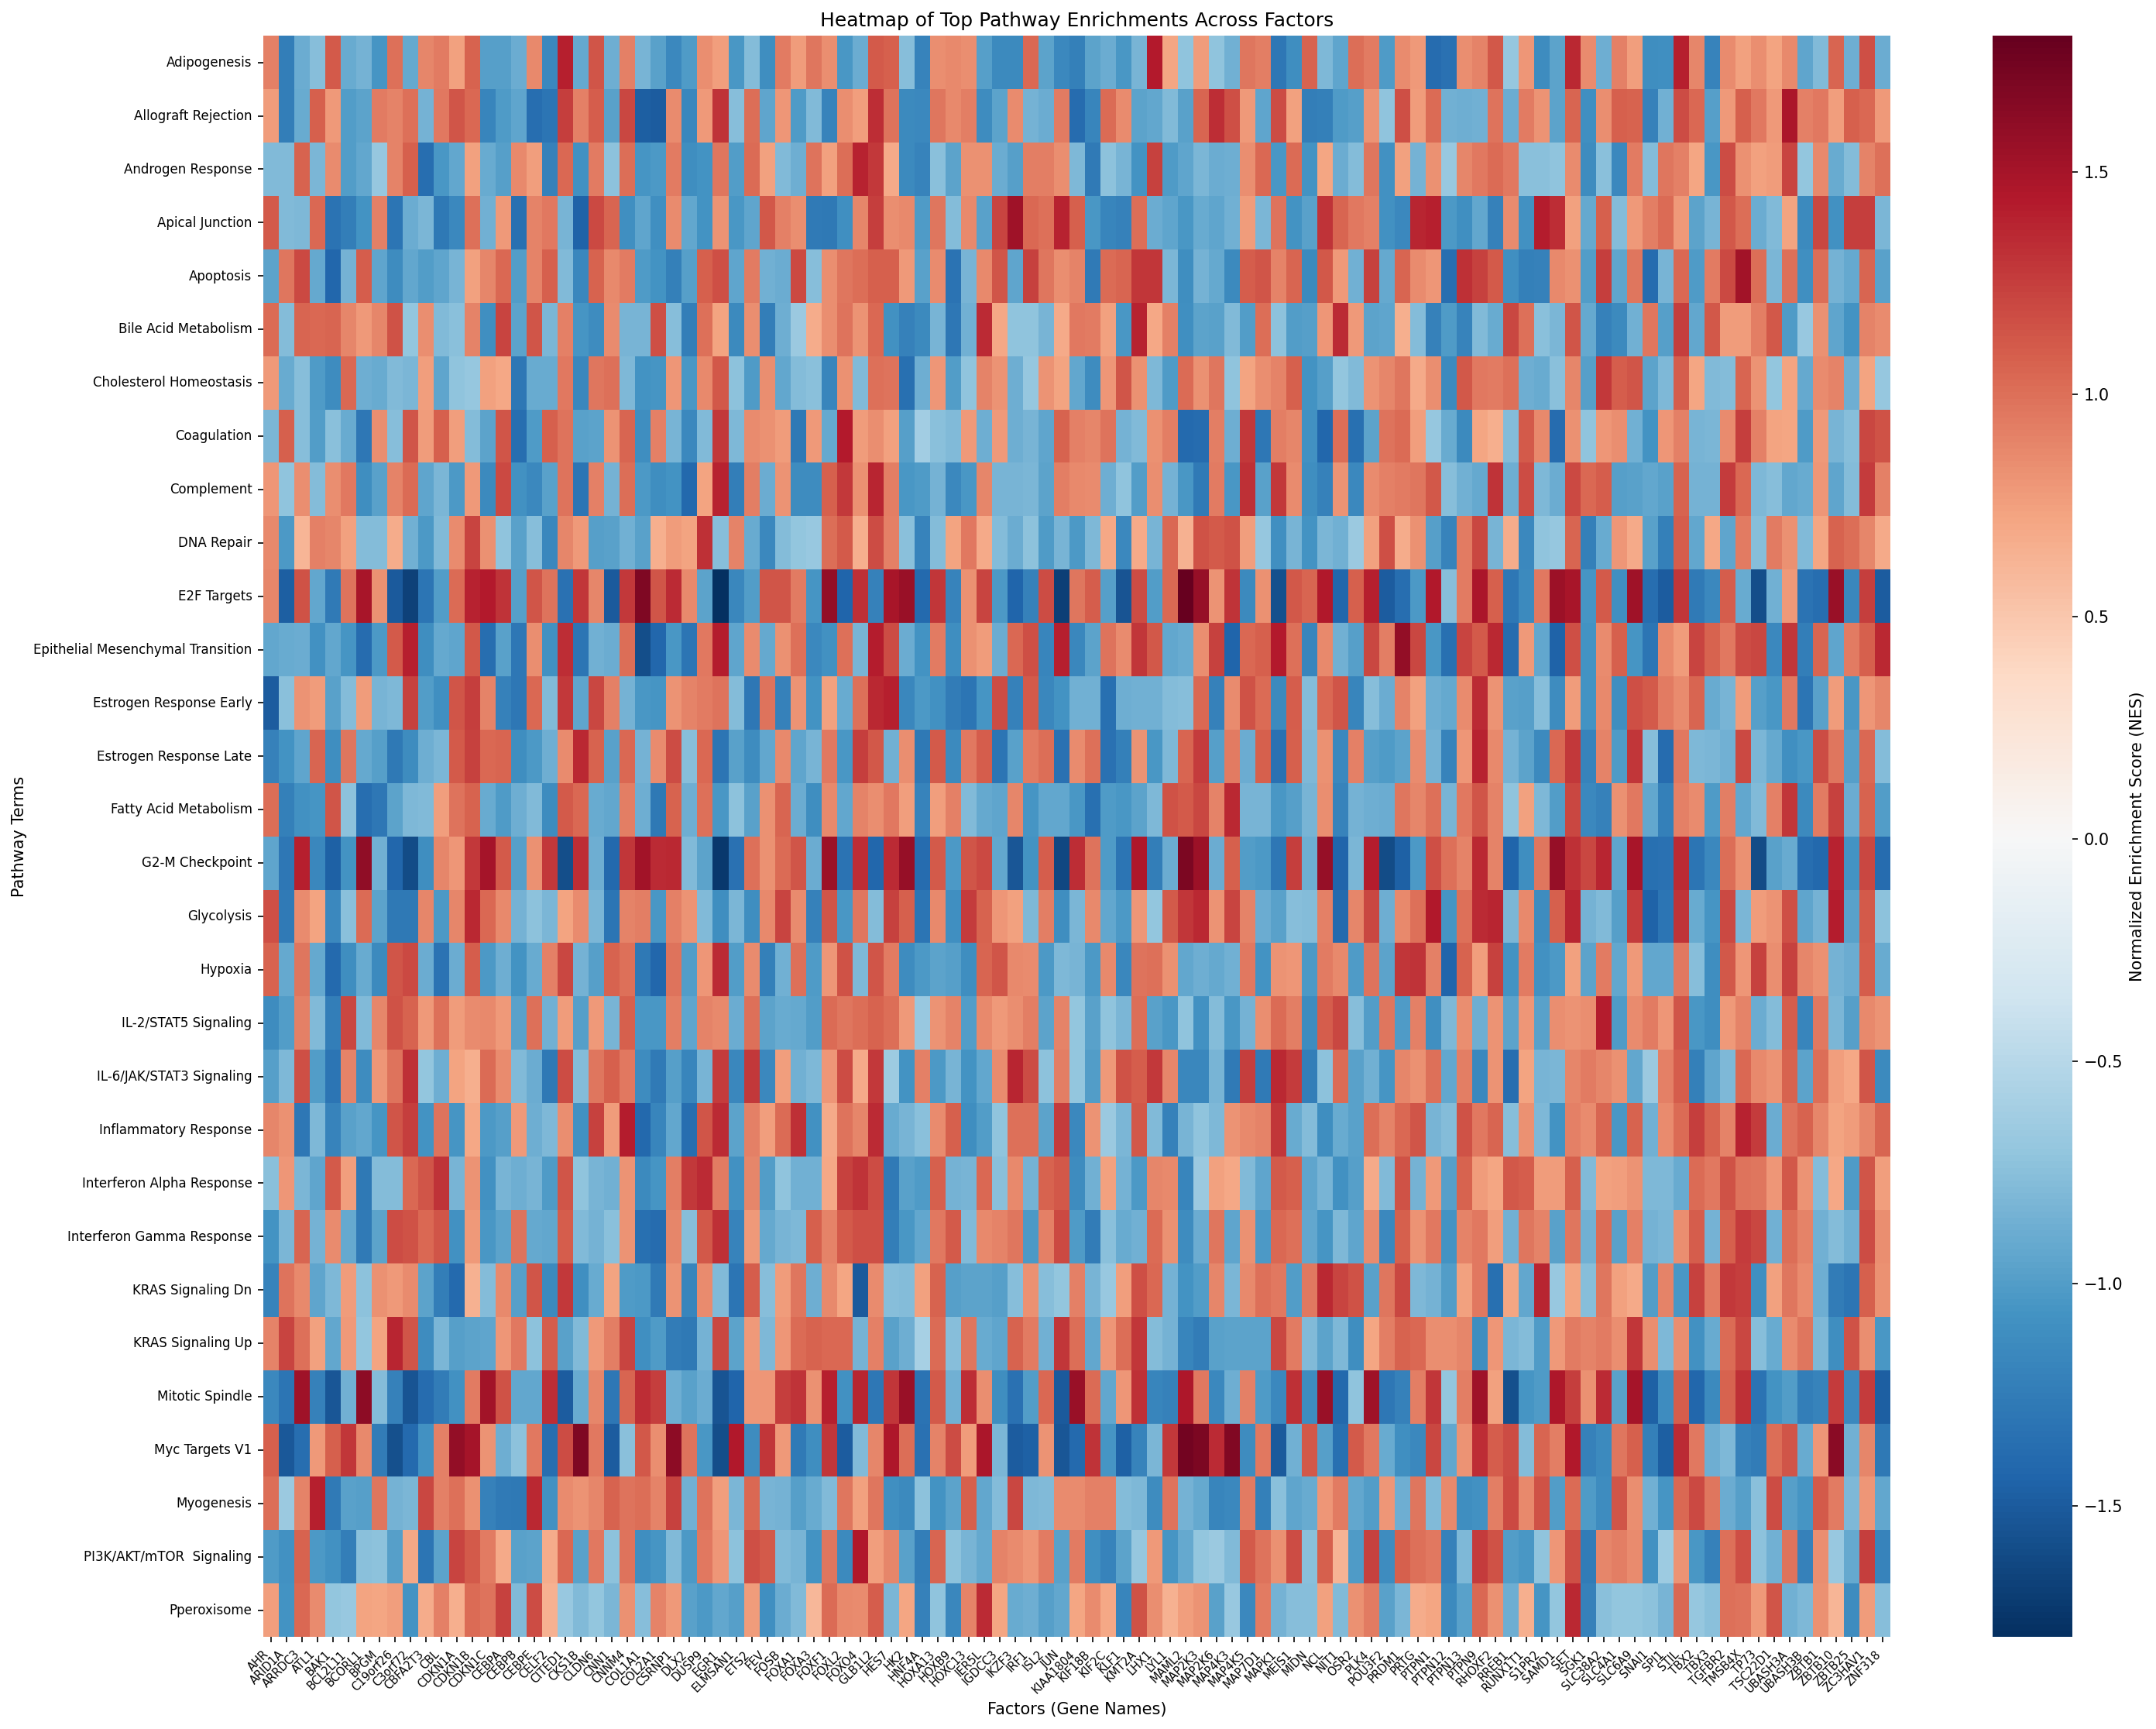
\includegraphics[width=\textwidth]{gfx/results/pathway_enrichment_heatmap.png}
    \caption{\revised{Heatmap of Top Pathway Enrichments Across Learned \cmps{}. 
    Each column corresponds to a specific \cmp{} ($z_i$) in the \gls{raptorgraph} model. Importantly, these labels are not post-hoc assignments; due to the GraphPathway encoder's preconditioning, each \cmp{} $z_i$ is architecturally constrained to mediate the effect of a specific gene perturbation (labeled on the x-axis).
    The rows represent biological pathways from the MSigDB Hallmark collection. The color intensity indicates the Normalized Enrichment Score (NES) derived from in-silico perturbation of that factor. The strong concordance between the architectural label and the biological result confirms that the model has successfully encoded the specific biological function of each gene into its corresponding \cmp{}.}}
    \label{fig:app:pathway_heatmap_supp}
\end{figure}

\revised{The GSEA analysis reveals that \gls{raptorgraph} captures distinct and biologically accurate programs. \Cref{fig:app:pathway_heatmap_supp} and \Cref{fig:rebuttal:gsea_dots} visualize the Normalized Enrichment Scores (NES) for the top enriched pathways across the learned factors. We highlight distinct biological programs captured by the model, verified against the known functions of their corresponding gene perturbations:}
\begin{enumerate}
    \item \revised{\textbf{Differentiation-Induced Arrest:} The \cmp{} linked to \textit{EGR1} displays massive negative enrichment for ``E2F Targets'' (NES $-1.79$, FDR $\approx 0.0$) and ``G2-M Checkpoint'' (NES $-1.72$, FDR $\approx 0.0$).
    EGR1 is a known tumor suppressor in K562 leukemia cells that drives differentiation along the megakaryocytic lineage, a process that necessitates a complete exit from the cell cycle \citep{ma_emodin_2019}.
    \gls{raptorgraph} correctly identifies this potent anti-proliferative program.}
    \item \revised{\textbf{Stress-Induced Growth Arrest:} The \cmp{} linked to the AP-1 subunit \textit{JUN} shows strong negative enrichment for ``E2F Targets'' (NES $-1.69$, FDR $< 0.001$) and ``G2-M Checkpoint'' (NES $-1.63$, FDR $< 0.002$). While often associated with inflammation, c-Jun is a central stress-response mediator; in the context of K562 cells, its activation drives a termination of cell division required for stress adaptation or differentiation \citep{shaulian_ap-1_2002, shaulian_mammalian_2000}.}
    \item \revised{\textbf{p53-Like Tumor Suppression:} The \cmp{} associated with \textit{TP73} displays significant negative enrichment for ``G2-M Checkpoint'' (NES $-1.60$, FDR $< 0.03$).
    \textit{TP73} is a functional homolog of \textit{TP53} (p53); its activation triggers downstream checkpoint signaling that arrests the cell cycle to prevent genomic instability \citep{kaghad_monoallelically_1997}.}
\end{enumerate}

\revised{
These findings confirm that the nodes in our learned DAG represent specific, identifiable biological mechanisms.
Consequently, the edges learned by the DAGMA module can be interpreted as causal regulatory links between these verified biological processes.
A detailed description of the methodology is provided in \cref{app:metrics:gsea_setup}.
}

%===============================================================================
\subsection{\revised{Extended Results: Computational Complexity of Optimal Transport Preprocessing}}
\label{app:extended_results:ot_complexity}
%===============================================================================

\revised{
    % \paragraph{Theoretical Complexity and Mitigation}
    We evaluated the computational cost of the proposed \gls{ot} pairing strategy compared to a random baseline. While random pairing scales linearly ($O(N)$), the \gls{ot} approach involves solving the \gls{emd} problem, which typically exhibits a worst-case complexity of $O(N^3 \log N)$. 
}

\revised{
    To mitigate this, the \gls{ot} pairing problem is formulated by taking the entire control population ($N_{ctrl} = 8,907$) and pairing it independently with each specific intervened population (i.e., cells sharing the same perturbation label, $N_k$ in the hundreds). 
    This effectively segments the total perturbed dataset ($N = 108,497$) into many smaller, manageable \gls{ot} problems, significantly reducing the $N$ in the $O(N^3 \log N)$ complexity for each individual transport plan and enabling efficient parallelization.
}

\revised{
    % \paragraph{Empirical Performance Benchmarks}
    We quantified the overhead of \gls{ot} preprocessing on a workstation equipped with an Intel Core i9-9900K CPU (8 cores, 16 threads) and 64 GB RAM.
    The \gls{ot} preprocessing added approximately 34 seconds to the baseline execution time (Random: 1m 44s vs. \gls{ot}: 2m 18s). 
    Detailed profiling confirmed that the process is compute-bound but highly efficient:
    \begin{itemize}
        \item \textbf{Parallelization}: The process achieved a peak CPU utilization of 1140\%, confirming that the the strategy effectively saturates available cores ($\approx 11.4$ active threads).
        \item \textbf{Memory}: Peak memory usage was modest at 2.4 GB.
    \end{itemize}
}

\revised{
    % \paragraph{Contextual Overhead on GPU Training}
    To contextualize this cost, we benchmarked the total training time for a standard 100-epoch experiment on an NVIDIA RTX 3090 GPU ($\approx 25.8$ minutes). The 34-second \gls{ot} overhead represents only 2.2\% of the total experimental runtime. Given that \gls{ot} is critical for preserving causal identifiability and preventing mean collapse, this negligible computational cost presents a highly favorable trade-off.
}

\newpage

%===============================================================================
\subsection{\revised{Extended Results: Empirical Analysis of Loss Functions for Sparse Single-Cell Causal Inference}}
\label{app:extended_results:loss_function_analysis}
%===============================================================================

\revised{
% \subsubsection{Motivation}
Training causal inference models on \gls{scRNAseq} data presents unique challenges due to two fundamental properties of the data: high sparsity and the lack of paired ground truth observations (unpaired control and perturbed populations).
To address this, we utilize \gls{ot} as a preprocessing step to infer latent couplings, combined with \gls{mmd} or reconstruction losses. 
}

\revised{
To rigorously demonstrate the necessity of this approach compared to baselines (e.g., Random Pairing or \gls{mmd}-only objectives), we conducted an empirical ablation study using synthetic data. 
This controlled environment allows us to overcome the ``missing pair'' problem inherent in real biological data, where the lack of ground truth counterfactuals makes it impossible to definitively validate causal alignment.
The code to reproduce these results is available in our source code.
}

\revised{
% \paragraph{Rationale for Synthetic Data}
We utilized synthetic data for this analysis for three critical reasons:
\begin{enumerate}
    \item \textbf{Unobservable Counterfactuals:} In real \gls{scRNAseq}, measuring a cell destroys it, making it impossible to observe the same cell in both control and perturbed states ($x_i$ and $y_i$). Synthetic data allows us to fabricate ground truth pairs, providing access to latent ground truth to definitively quantify causal accuracy.
    \item \textbf{Controlled Sparsity Sweep:} Real data has fixed, high sparsity. Synthetic data allows us to sweep sparsity from $0\%$ to $99\%$ to empirically observe the phase transition where reconstruction metrics degrade.
    \item \textbf{Signal Isolation:} It allows us to isolate the mathematical properties of the loss functions from biological noise and batch effects.
\end{enumerate}
}

\revised{
% \subsubsection{Experimental Setup}
% \textbf{Data Generation:}
We simulated a dataset of 1000 samples with 5000 features (genes).
\begin{itemize}
    \item \textbf{Control Population ($X$):} Generated from $\mathcal{N}(0, 1)$ and masked to achieve target sparsity levels ranging from $0\%$ to $99\%$.
    \item \textbf{Perturbation:} A systematic shift was added to the first 50 features ($+2.0$) to simulate a biological effect.
    \item \textbf{Ground Truth ($Y$):} The perturbed state for each control cell, preserving the sparse structure.
\end{itemize}
}

\revised{
% \textbf{Comparison Scenarios:}
We evaluated three hypothetical model outputs against the ground truth $Y$, representing the outcomes of different training strategies:
\begin{enumerate}
    \item \textbf{Causal/Paired Model (Ideal):} The ground truth $Y$ with added Gaussian noise ($\sigma=0.1$). 
    \textit{Representation:} This proxies the outcome of a model trained with \gls{ot}-based pairing.
    By recovering the latent pairs ($x_i \to y_i$), the model learns the correct cell-specific trajectories.
    \item \textbf{Population/Generative Model (Unpaired):} The ground truth population $Y$ with sample indices randomly permuted.
    This proxies the equilibrium state of a model trained with \gls{mmd} only.
    Such a model perfectly matches the target distribution $P(Y)$ (minimizing the \gls{mmd} loss) but fails to learn the causal mapping ($f(x_i) \neq y_i$), effectively becoming a generative model of the population rather than a causal predictor.
    \item \textbf{Mode Collapse (Average):} The mean vector $\bar{Y}$ repeated for all samples.
    This represents the failure mode of Random Pairing (\gls{mse}).
    When training on random pairs, the model minimizes variance by predicting the population mean.
\end{enumerate}
}

\revised{
% \textbf{Metrics Evaluated:}
We evaluated three metrics in this extended results:
\begin{itemize}
    \item \textbf{\gls{mse}:} Standard point-wise reconstruction loss.
    \item \textbf{\gls{mmd}:} Distributional distance using a multi-scale Gaussian kernel.
    \item \textbf{\gls{ot}:} Exact \gls{emd} (Wasserstein-2).
\end{itemize}
}

\revised{
\subsubsection{Results}
We evaluated the metrics across varying sparsity levels (see \Cref{tab:metric_ablation}) to identify the failure modes of standard losses.
}

\revised{
\begin{table}[ht]
\centering
\caption{
    Metric Performance Across Sparsity Regimes. Lower is better.
    Bold indicates the metric's ``preferred'' model.
}
\label{tab:metric_ablation}
\begin{tabular}{llcccc}
\toprule
\multirow{2}{*}{\textbf{Sparsity}} & \multirow{2}{*}{\textbf{Metric}} & \textbf{Causal/Paired} & \textbf{Population/Generative} & \textbf{Mode Collapse} & \multirow{2}{*}{\textbf{Verdict}} \\
& & (\gls{ot}+\gls{mmd}) & (\gls{mmd} Only) & (\gls{mse} Failure) & \\
\midrule
\textbf{0\%} & \textbf{\gls{mse}} & $\mathbf{0.0100}$ & $1.9947$ & $1.0000$ & \textbf{Success.} \\
(Dense) & \textbf{\gls{mmd}} & $\mathbf{-0.0061}$ & $\mathbf{-0.0062}$ & $2.3127$ & \textbf{Ambiguity.} \\
\midrule
\textbf{50\%} & \textbf{\gls{mse}} & $\mathbf{0.0100}$ & $0.9987$ & $0.4989$ & \textbf{Degradation.} \\
(Medium) & \textbf{\gls{mmd}} & $-0.0059$ & $\mathbf{-0.0062}$ & $2.3119$ & \textbf{Failure.} \\
\midrule
\textbf{90\%} & \textbf{\gls{mse}} & $\mathbf{0.0100}$ & $0.1997$ & $0.0997$ & \textbf{Weakness.} \\
(High) & \textbf{\gls{mmd}} & $-0.0022$ & $\mathbf{-0.0062}$ & $2.3066$ & \textbf{Failure.} \\
\midrule
\textbf{99\%} & \textbf{\gls{mse}} & $0.0100$ & $0.0201$ & $\mathbf{0.0101}$ & \textbf{Failure.} \\
(Extreme) & \textbf{\gls{mmd}} & $0.1648$ & $\mathbf{-0.0061}$ & $2.2505$ & \textbf{Failure.} \\
& \textbf{\gls{ot}} & $49.95$ & $\mathbf{0.00}$ & $50.26$ & \textbf{Failure.} \\
\bottomrule
\end{tabular}
\end{table}
}

\revised{
% \paragraph{Failure of \gls{mmd}-Only Objectives (Identifiability Failure)}
The most critical finding is observed in the ``Population/Generative'' column. Across all sparsity levels, \gls{mmd} assigns a perfect or near-perfect score ($\approx 0.0$) to the Population Model.
This implies that a model trained with \gls{mmd} as the sole objective has no incentive to learn the correct causal mapping. It can achieve zero loss simply by generating a realistic population that is causally scrambled (i.e., Control Cell A is mapped to Perturbed State B). The result is that the model learns the \textit{distribution} but loses the \textit{cell identity}.
}

\revised{
% \paragraph{Failure of Random Pairing (Convergence to Mean)}
Even if we attempted to force pairing using standard reconstruction (\gls{mse}), the high sparsity (99\%) causes \gls{mse} to favor the Mode Collapse ($0.0101$) over the correct structure ($0.0100$). This empirically demonstrates that training on random pairs forces the model to converge to the population mean, which on sparse data is indistinguishable from a valid prediction in terms of error magnitude.
}

\revised{
% \subsubsection{Conclusion: The Necessity of \gls{ot} Preprocessing}
The empirical results provide definitive proof that standard approaches are insufficient for sparse, unpaired causal inference:
\begin{enumerate}
    \item \textbf{\gls{mmd}-Only Training} leads to Causal Scrambling (Permutation Invariance).
    \item \textbf{Random Pairing / \gls{mse} Training} leads to Mode Collapse (Convergence to Mean).
\end{enumerate}
This justifies the necessity of \textbf{\gls{ot} preprocessing}. By solving for the optimal coupling matrix $\pi$ that minimizes transport cost, we explicitly enforce the Principle of Minimal Action, assuming that cells undergo the smallest necessary transcriptomic change. This effectively infers the latent pairing that \gls{mse} assumes exists, resolving the identifiability crisis that \gls{mmd} ignores and avoiding the collapse mode that Random Pairing induces.
}

%===============================================================================
\subsection{\revised{Extended Results: Impact of Optimal Transport on Downstream Tasks}}
\label{app:extended_results:ot_impact}
%===============================================================================

\revised{
% \subsubsection{Motivation}
While the primary motivation for integrating \gls{ot} is to prevent mean collapse and preserve population structure during training, its ultimate value lies in improving performance on downstream biological tasks.
We conducted an ablation study comparing the standard \gls{ot}-based pairing against a Random Pairing baseline to isolate the impact of this preprocessing step on the model's ability to predict non-additive genetic interactions.
}

\revised{
% \subsubsection{Genetic Interaction Prediction}
We evaluated both models on the ``Genetic Interaction'' benchmark (Precision @ 10).
As shown in \Cref{tab:ot_ablation_gi}, the inclusion of \gls{ot} leads to a marked improvement in identifying complex interaction types, specifically Redundancy, Epistasis, and Suppression.
}

\revised{
\begin{table}[ht]
\centering
\caption{
    Ablation Study: Impact of Optimal Transport on Genetic Interaction Prediction (Precision @ 10).
    The model trained with \gls{ot} preprocessing consistently outperforms the Random Pairing baseline in detecting complex interaction types (Redundancy, Epistasis, Suppression), demonstrating that OT helps preserve the fine-grained causal structure required for these tasks.
}
\label{tab:ot_ablation_gi}
\begin{tabular}{lcc}
\toprule
\textbf{Interaction Type} & \textbf{Random Pairing} & \textbf{Optimal Transport} \\
\midrule
Neomorphism & 0.4 & 0.4 \\
Redundancy & 0.7 & \textbf{0.8} \\
Epistasis & 0.8 & \textbf{0.9} \\
Synergy & \textbf{0.5} & 0.4 \\
Suppression & 0.2 & \textbf{0.3} \\
\bottomrule
\end{tabular}
\end{table}
}

\revised{
% \subsubsection{Analysis}
The results indicate that while Random Pairing can achieve competitive performance on simpler metrics (like Neomorphism), it falls short in capturing the subtle dependencies required to identify Redundancy and Epistasis.
The \gls{ot} pairing, by matching cells based on their distributional similarity, likely preserves the underlying biological signal that defines these interactions, preventing them from being washed out by the noise of random assignment.
This validates the hypothesis that \gls{ot} is not just a theoretical necessity for causal identifiability but a practical enhancer of model utility for complex biological discovery.
}

%===============================================================================
\subsection{\revised{Extended Results: Ablation Study on $\beta$-VAE and DAGMA Regularization}}
\label{app:extended_results:ablation_study}
%===============================================================================

\revised{
% \subsubsection{Introduction and Motivation}
The primary goal of this ablation study is to rigorously assess the sensitivity of the RAPTORGraph model to its key regularization parameters, specifically the $\beta$ parameter of the $\beta$-VAE ($\beta$) and the weights of the DAGMA loss ($\mu$ and $\lambda_1$). Our core hypotheses for this study were: 1. The criticality of $\beta$ for preventing mode collapse, where we investigated if $\beta$ is the most crucial hyperparameter for maintaining a regularized and informative latent space, looking for evidence of KL divergence approaching zero and its detrimental effects on learning meaningful representations. 2. The hierarchy of hyperparameter importance, testing the assertion that $\beta$ is of primary importance, followed by the DAGMA weights, in terms of their impact on downstream performance.
}

\revised{
% \subsubsection{Methodology}
The study was conducted using the RAPTORGraph model on the Norman et al. 2019 dataset. For the hyperparameter sweep, $\beta$ was swept across {0.0, 0.1, 0.4, 0.8, 1.2, 1.6, 2.0, 2.5, 3.0} to observe its effect on KL divergence and to test for mode collapse. Additionally, $\mu$ and $\lambda_1$ were varied around default values to analyze their influence on the causal graph structure, specifically $\mu \in \{0.1, 0.27, 0.5\}$ and $\lambda_1 \in \{0.02, 0.05, 0.1\}$. The evaluation metrics included: a) KL Divergence as the primary metric to monitor for signs of mode collapse; b) Prediction Variance (Pred. Var.), representing the variance of the reconstructed gene expression for \textit{control} cells, used to detect mean collapse; and c) \gls{mmd} to evaluate the quality of predictions for \textit{intervened or perturbed} cells. Notably, \gls{mse} is not explicitly used for mode collapse detection in this context, as variance directly assesses the diversity of generated outputs, which \gls{mse} alone might obscure.
% To better visualize the dominant effect of $\beta$ on the latent space, Table~ef{\ref{tab:ablation_consolidated}} summarizes all experiments. The goal is to demonstrate that $\beta$ is the primary factor driving the KL divergence towards zero regardless of the DAGMA hyperparameter settings, indicating posterior collapse.
}

\revised{
% \subsubsection{Experiment and Analysis}
To better visualize the dominant effect of $\beta$ on the latent space, \Cref{tab:ablation_consolidated} summarizes all experiments. The goal is to demonstrate that $\beta$ is the primary factor driving the KL divergence towards zero regardless of the DAGMA hyperparameter settings, indicating posterior collapse.
}

\begin{table}[ht]
\small
\centering
\caption{
    \revised{Impact of $\beta$-VAE and DAGMA Regularization on Model Performance. 
    \textbf{Pred. Var.} denotes the variance of the predicted cell states (or variance of predicted control cells), where a lower value may indicate mean collapse. 
    Lower \gls{mmd} indicates better distribution matching. 
    The bold row indicates the selected best configuration.}
}
\label{tab:ablation_consolidated}
% \resizebox{\textwidth}{!}{
\begin{tabular}{cccccc}
\toprule
\textbf{$\beta$} & \textbf{$\mu$} & \textbf{$\lambda_1$} & \textbf{KL Divergence} & \textbf{Pred. Var.} & \textbf{\gls{mmd}} \\
\midrule
0.0 & 0.27 & 0.052 & 0.0181 & 0.0181 & 1.929 \\
\midrule
0.1 & 0.1 & 0.02 & 0.059 & 0.0059 & 0.268 \\
0.1 & 0.1 & 0.05 & 0.058 & 0.0067 & 0.257 \\
0.1 & 0.1 & 0.1 & 0.054 & 0.0073 & 0.161 \\
0.1 & 0.27 & 0.02 & 0.061 & 0.0051 & 0.401 \\
0.1 & 0.27 & 0.05 & 0.060 & 0.0062 & 0.318 \\
0.1 & 0.27 & 0.1 & 0.0615 & 0.0068 & 0.209 \\
0.1 & 0.5 & 0.02 & 0.0609 & 0.0048 & 0.510 \\
0.1 & 0.5 & 0.05 & 0.0604 & 0.0054 & 0.450 \\
0.1 & 0.5 & 0.1 & 0.0572 & 0.0058 & 0.319 \\
\midrule
0.4 & 0.1 & 0.02 & 0.0040 & 0.0010 & 0.120 \\
0.4 & 0.1 & 0.05 & 0.0039 & 0.0010 & 0.117 \\
0.4 & 0.1 & 0.1 & 0.0040 & 0.0009 & 0.117 \\
0.4 & 0.27 & 0.02 & 0.0040 & 0.0009 & 0.133 \\
\textbf{0.4} & \textbf{0.27} & \textbf{0.05} & \textbf{0.0039} & \textbf{0.0009} & \textbf{0.127} \\
0.4 & 0.27 & 0.1 & 0.0040 & 0.0008 & 0.121 \\
0.4 & 0.5 & 0.02 & 0.0040 & 0.0007 & 0.203 \\
0.4 & 0.5 & 0.05 & 0.0040 & 0.0007 & 0.196 \\
0.4 & 0.5 & 0.1 & 0.0040 & 0.0007 & 0.209 \\
\midrule
0.8 & 0.1 & 0.02 & 0.0009 & 0.0002 & 0.136 \\
0.8 & 0.1 & 0.05 & 0.0009 & 0.0002 & 0.132 \\
0.8 & 0.1 & 0.1 & 0.0009 & 0.0002 & 0.127 \\
0.8 & 0.27 & 0.02 & 0.0009 & 0.0002 & 0.147 \\
0.8 & 0.27 & 0.05 & 0.0009 & 0.0002 & 0.146 \\
0.8 & 0.27 & 0.1 & 0.0009 & 0.0002 & 0.143 \\
0.8 & 0.5 & 0.02 & 0.0008 & 0.0001 & 0.215 \\
0.8 & 0.5 & 0.05 & 0.0009 & 0.0001 & 0.227 \\
0.8 & 0.5 & 0.1 & 0.0009 & 0.0001 & 0.206 \\
\midrule
1.2 & 0.27 & 0.052 & 0.0003 & 0.00005 & 0.137 \\
1.6 & 0.27 & 0.052 & 0.0002 & 0.00002 & 0.144 \\
2.0 & 0.27 & 0.052 & 0.0001 & 0.00001 & 0.155 \\
2.5 & 0.27 & 0.052 & 0.0001 & 0.000007 & 0.171 \\
3.0 & 0.27 & 0.052 & 0.0000 & 0.000004 & 0.167 \\
\bottomrule
\end{tabular}
% }
\end{table}

\revised{
% \paragraph{Conclusion on Posterior Collapse}
The consolidated table makes the trend clear. For a given $\beta$ value (e.g., 0.4), the KL Divergence remains consistently low ($\approx 0.004$) across all variations of $\mu$ and $\lambda_1$. However, changing $\beta$ from 0.1 to 0.4, and then to 0.8 and higher, causes the KL Divergence to drop by orders of magnitude.
This demonstrates that $\beta$ is the determining factor for the degree of regularization and subsequent posterior collapse. The DAGMA weights have a negligible effect on the KL Divergence itself, reinforcing the conclusion that an appropriate $\beta$ must be selected first before fine-tuning the other parameters.
}

\revised{
% \paragraph{Selection of Best Configuration}
Our argument is to choose $\beta=0.4$ (approx. 0.447 in our final model) to balance the trade-off between distribution matching (\gls{mmd}) and preserving biological heterogeneity. The KL Divergence at this range ($\approx 1\times10^{-3}$) is chosen to be similar to baselines like dVAE and SENA, ensuring the model captures meaningful biological variability rather than regressing to the population mean. While $\beta=0.1$ preserves more variance, it suffers from poor stability and high \gls{mmd}. Conversely, $\beta=0.8$ achieves competitive \gls{mmd} but suffers from an order-of-magnitude drop in prediction variance ($1\times10^{-4}$ vs $1\times10^{-3}$), indicating severe over-smoothing. We select $\beta=0.4$ as the optimal operating point, minimizing \gls{mmd} while retaining significantly higher variance than the fully collapsed regimes. The bolded row in Table~\ref{tab:ablation_consolidated} represents this chosen configuration.
}

%===============================================================================
\subsection{\revised{Extended Results: Pairing Strategy Stability (n=7)}}
\label{app:extended_results:pairing_ablation}
%===============================================================================

\begin{figure}[H]
    \centering
    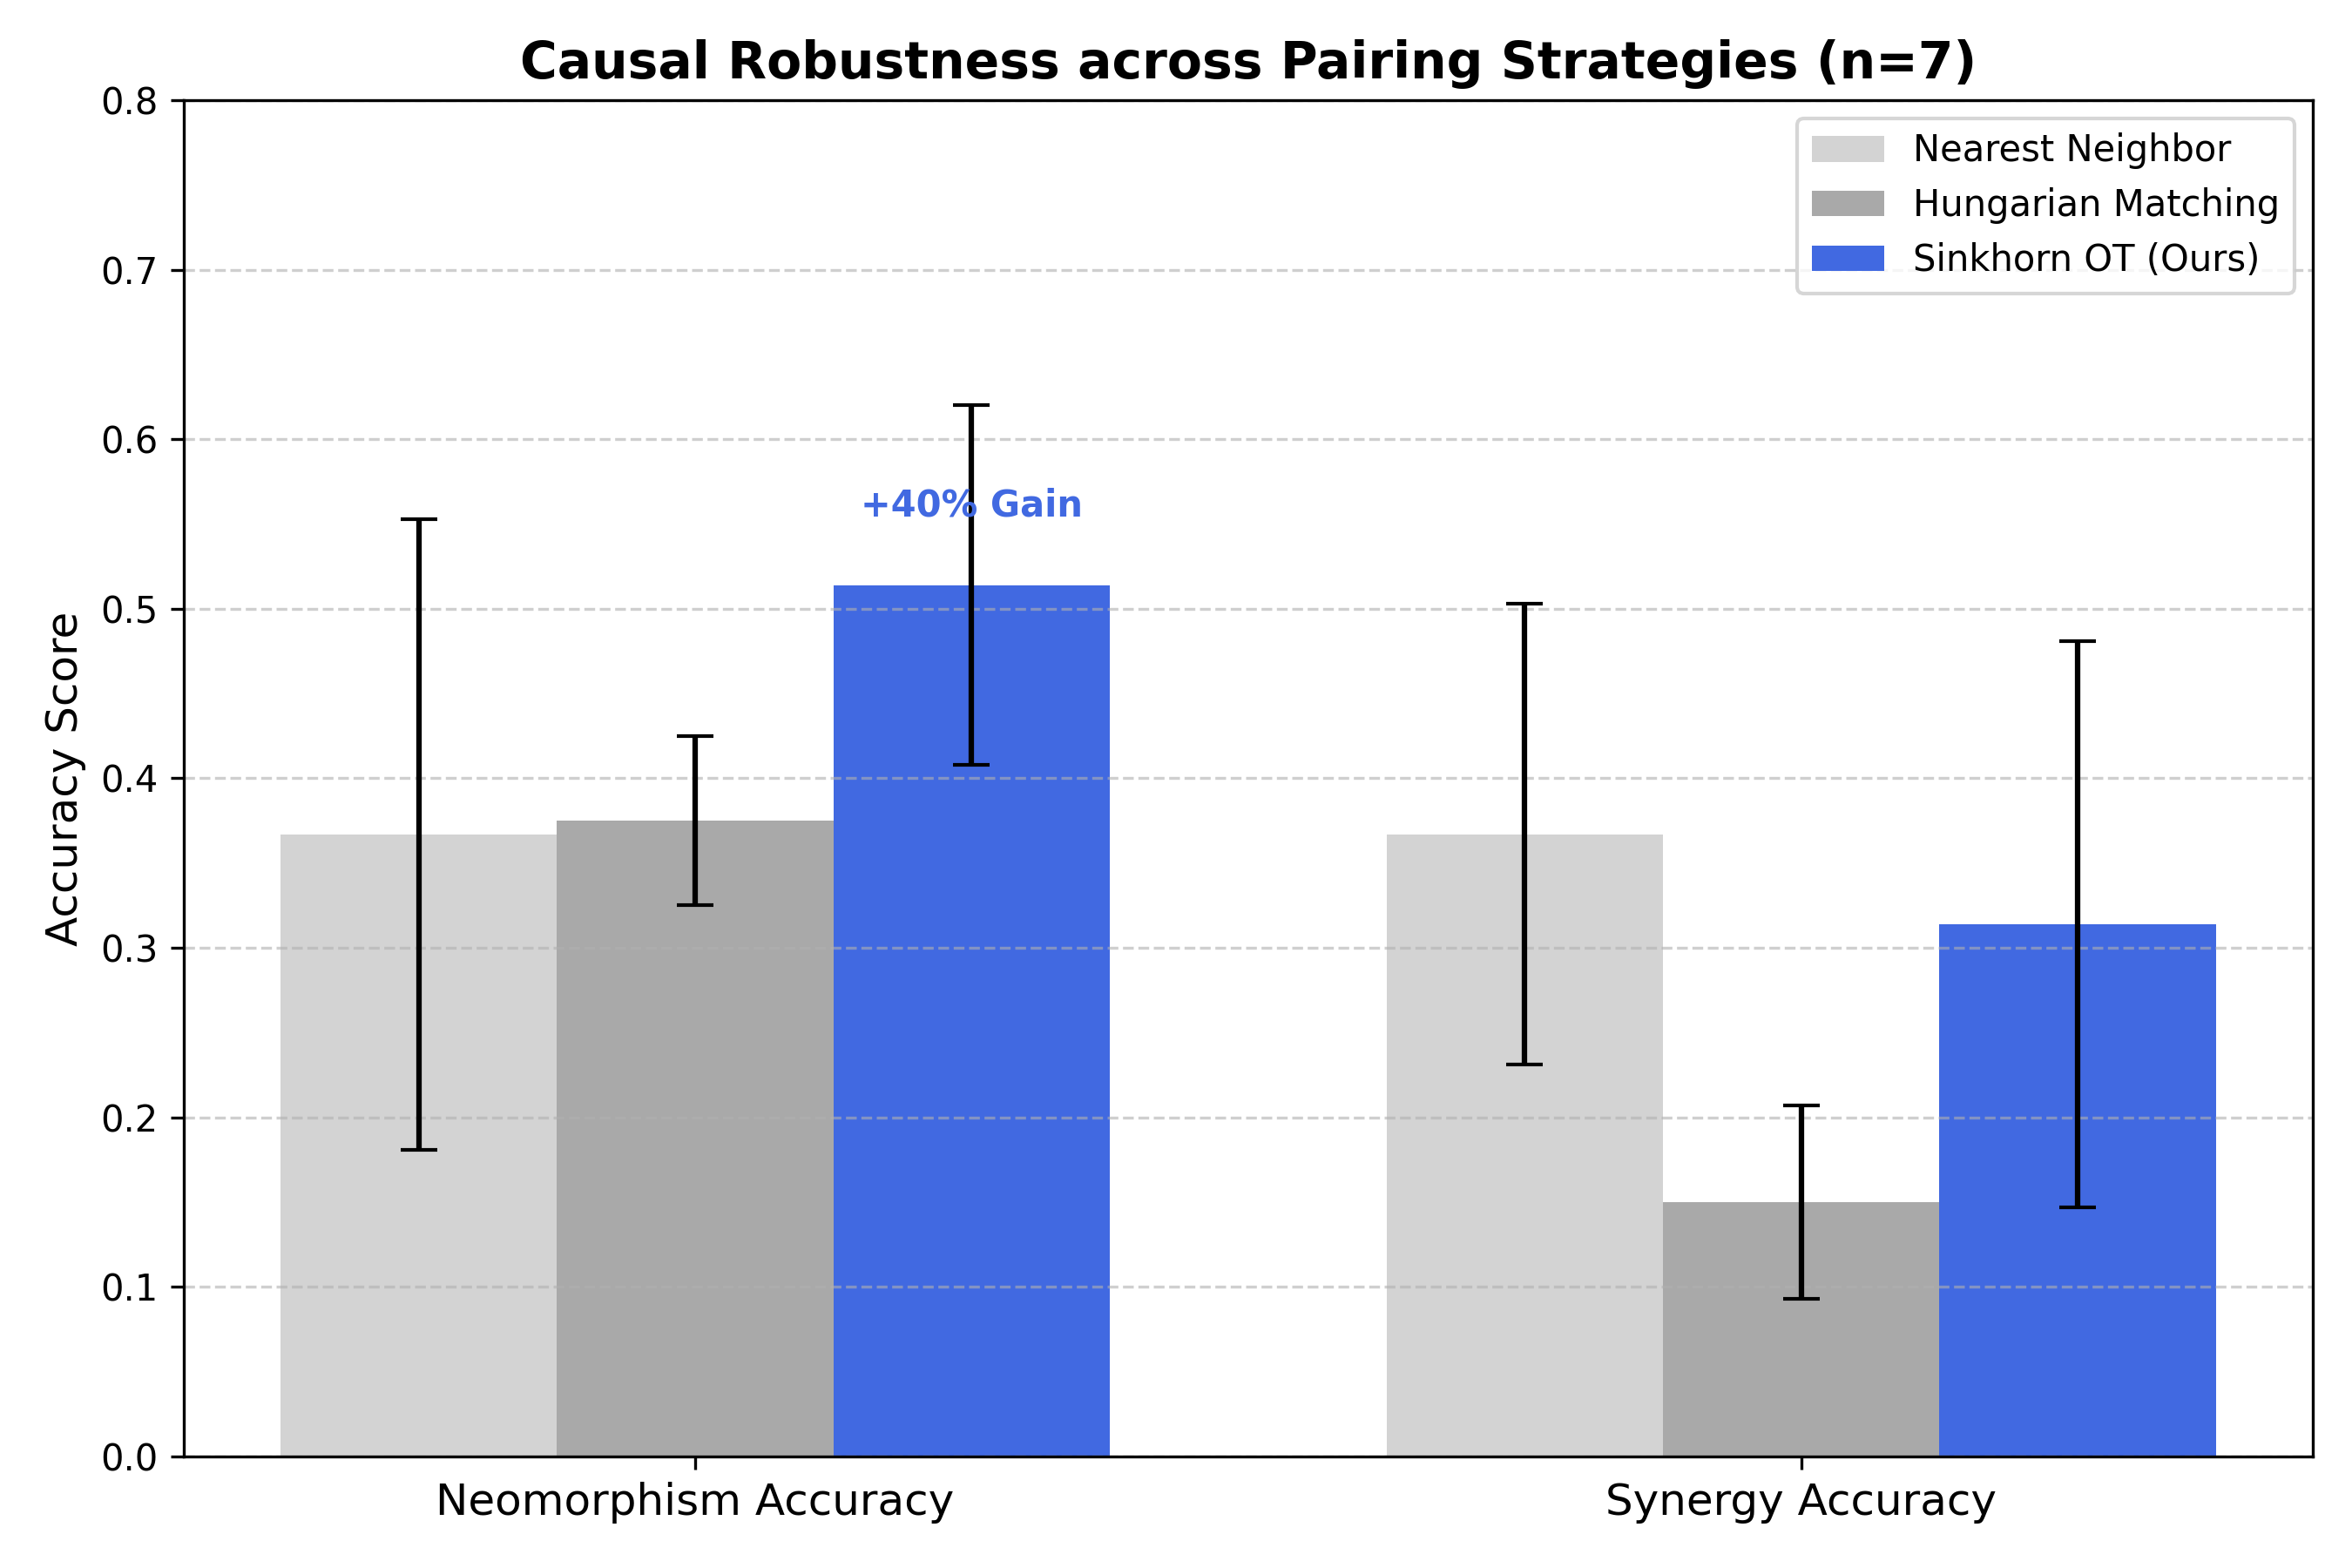
\includegraphics[width=0.8\textwidth]{gfx/rebuttal/fig_pairing_comparison.png}
    \caption{\revised{\textbf{Pairing Strategy Comparison ($n=7$).} Grouped bar chart demonstrating that Sinkhorn Optimal Transport (OT) significantly outperforms Nearest Neighbor and Hungarian matching in identifying synergistic and neomorphic effects.}}
    \label{fig:rebuttal:pairing_comparison}
\end{figure}

\revised{
We evaluate the impact of different cell-pairing strategies on the identification of Genetic Interactions (GI) across 7 independent seeds (\Cref{tab:app:pairing_ablation}). We compare Sinkhorn OT against Nearest Neighbor (NN) and Hungarian matching (see \cref{app:ot:alternatives} for technical definitions). Sinkhorn OT provides the most stable anchor, significantly outperforming NN by 40\% in Neomorphism identification.
}

\begin{table}[h]
\centering
\caption{\revised{\textbf{Pairing Strategy Comparison.} Metrics averaged over 7 independent seeds ($\pm$ SD).}}
\label{tab:app:pairing_ablation}
\begin{tabular}{lccc}
\toprule
Metric & Nearest Neighbor & Hungarian & \textbf{Sinkhorn OT} \\
\midrule
Unbiased MMD $\downarrow$ & 0.1243 $\pm$ 0.0350 & 0.4659 $\pm$ 0.0950 & \textbf{0.1161} $\pm$ 0.0630 \\
Neomorphism $\uparrow$ & 0.3667 $\pm$ 0.1860 & 0.3750 $\pm$ 0.0500 & \textbf{0.5143} $\pm$ 0.1060 \\
Synergy $\uparrow$ & 0.3667 $\pm$ 0.1360 & 0.1500 $\pm$ 0.0570 & \textbf{0.3143} $\pm$ 0.1670 \\
\bottomrule
\end{tabular}
\end{table}

%===============================================================================
\subsection{\revised{Extended Results: Sensitivity to Meta-Pathway Capacity}}
\label{app:extended_results:capacity_ablation}
%===============================================================================

\begin{figure}[H]
    \centering
    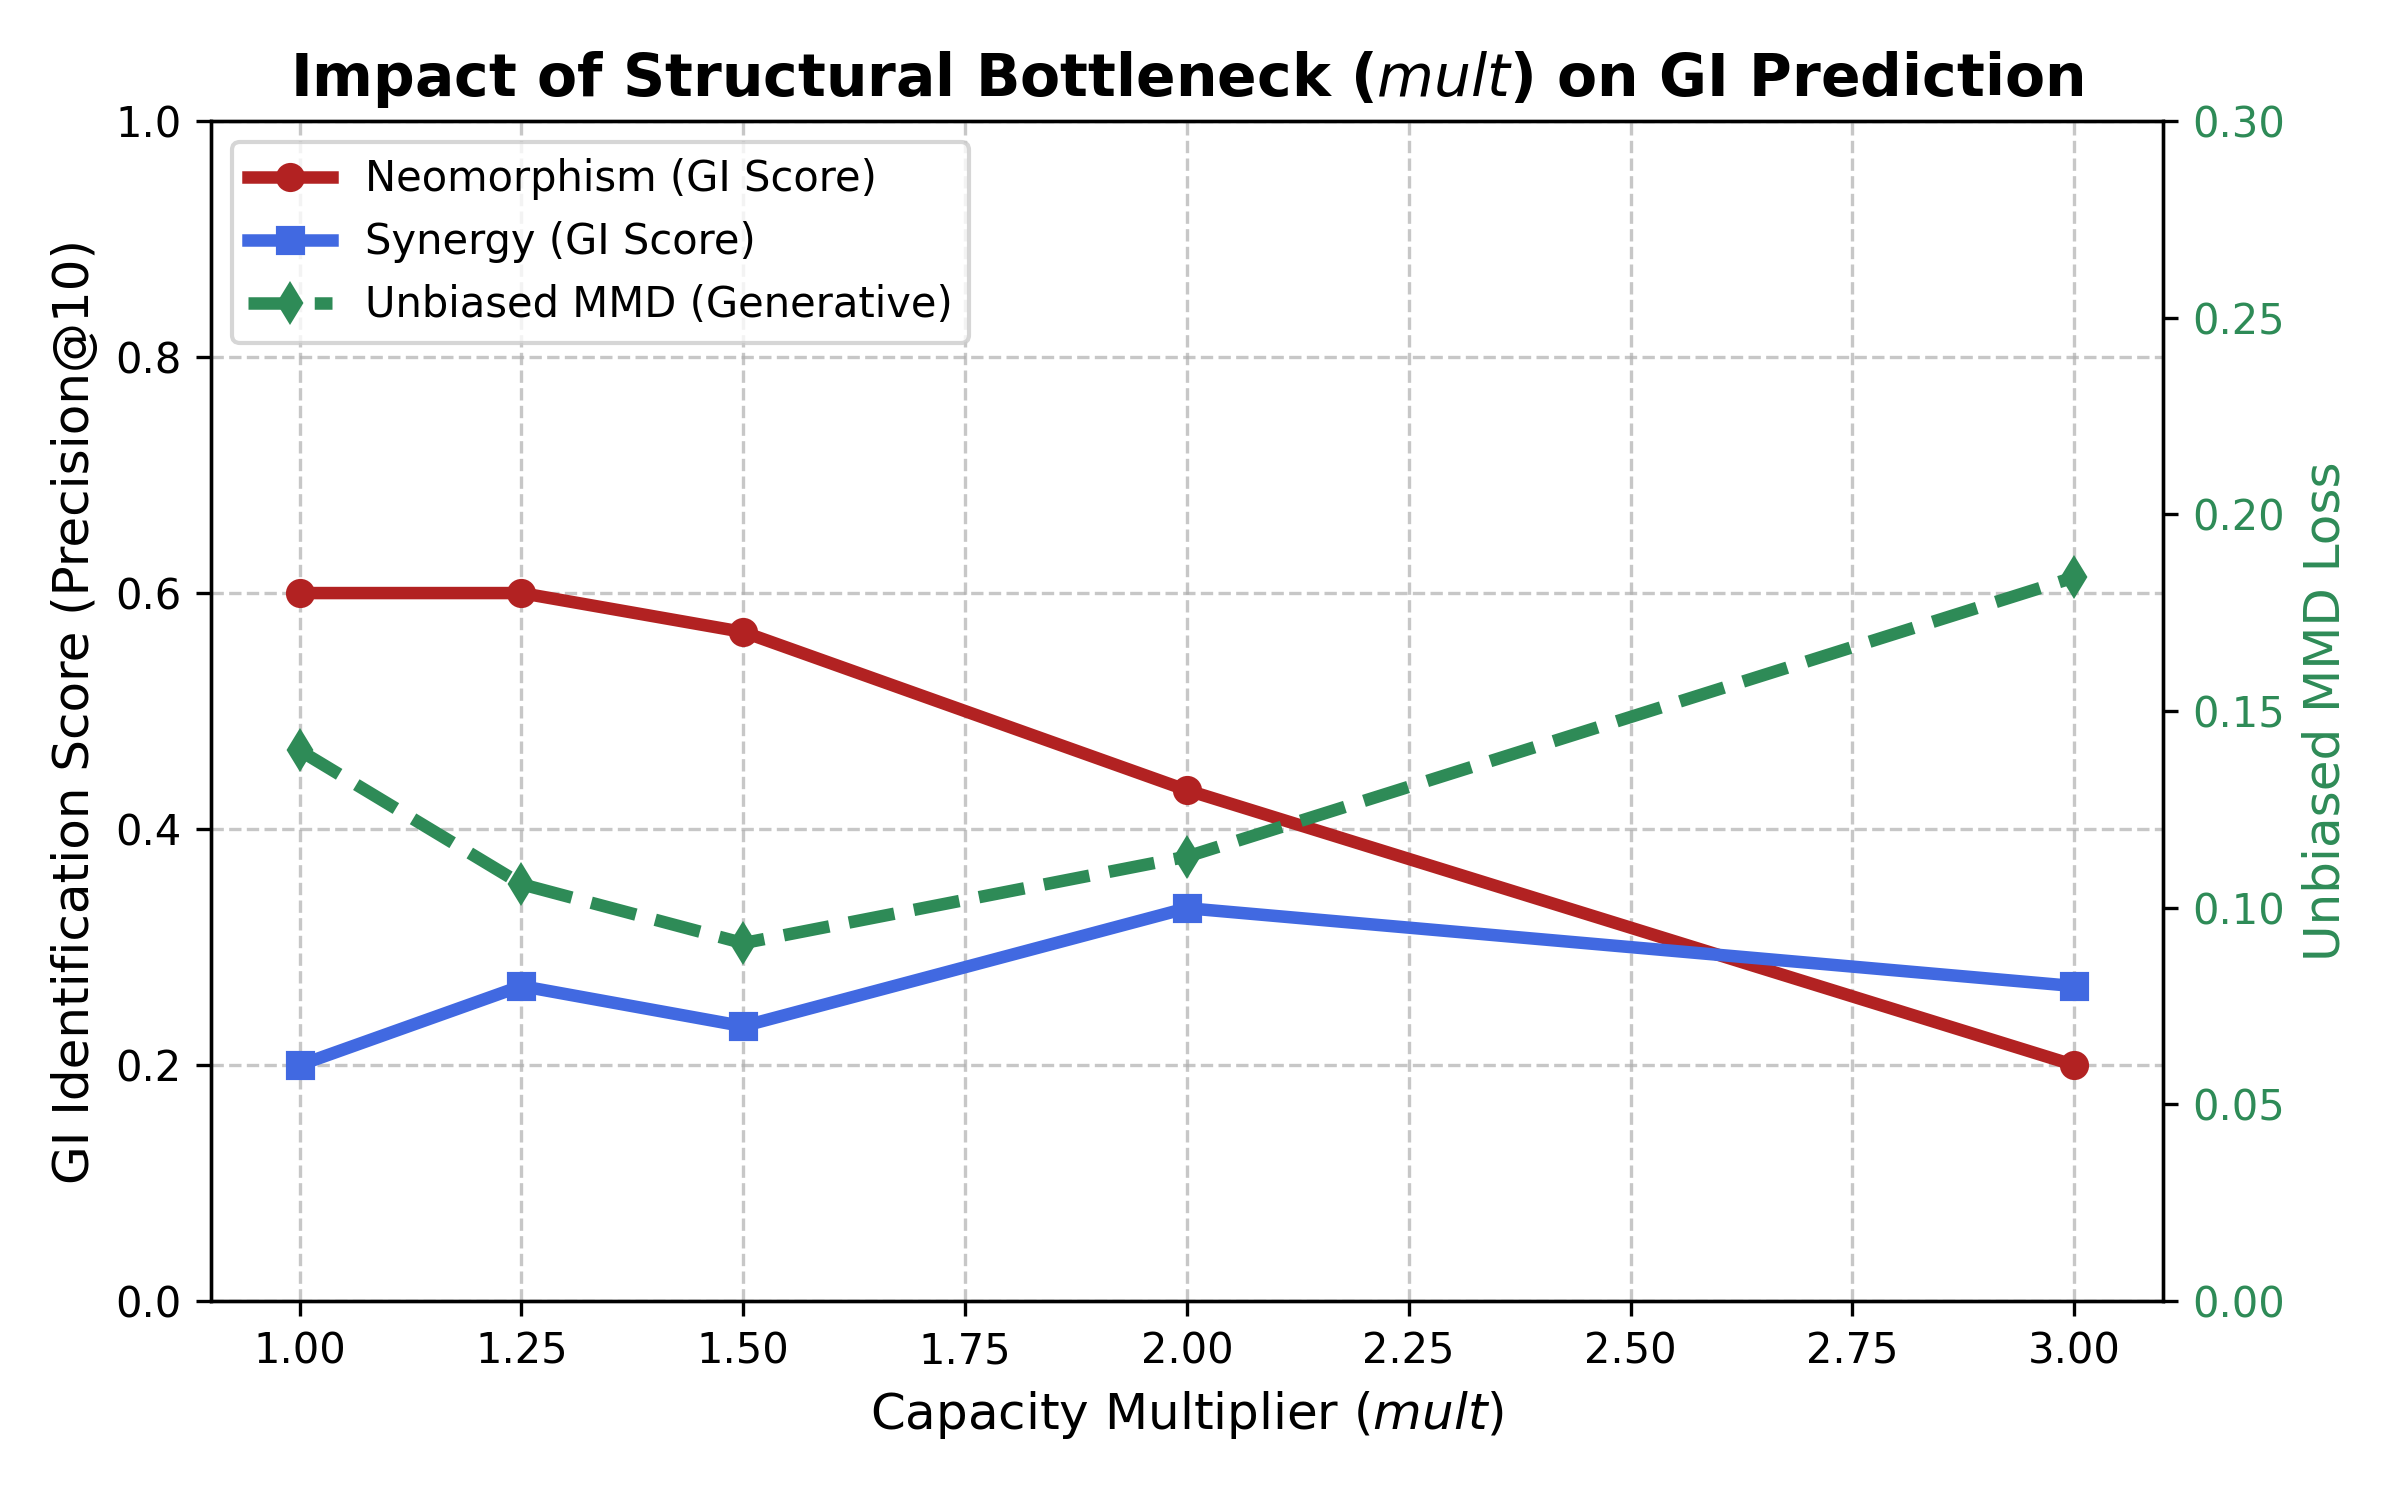
\includegraphics[width=0.8\textwidth]{gfx/rebuttal/fig_capacity_curve.png}
    \caption{\revised{\textbf{Impact of Structural Bottleneck ($mult$).} Performance metrics plotted as a function of the latent capacity multiplier. Peak causal performance is achieved at tight bottlenecks ($1.0-1.25$).}}
    \label{fig:rebuttal:capacity_curve}
\end{figure}

\revised{
To investigate the effect of the GraphPathway bottleneck, we define the parameter \textbf{$mult$}, representing the ratio of learned \cmps{} ($\latentdim$) to the number of known perturbed genes ($\numperturbedgenes$).
}

\begin{table}[h]
\centering
\caption{\revised{\textbf{Capacity Sweep Results.} Peak identification of **Genetic Interactions (GI scores)** occurs at tight structural bottlenecks. Results visualized in \cref{fig:rebuttal:capacity_curve}.}}
\label{tab:app:capacity_ablation}
\begin{tabular}{cccccc}
\toprule
Multiplier ($mult$) & 1.0 & 1.25 & 1.5 & 2.0 & 3.0 \\
\midrule
Neomorphism $\uparrow$ & \textbf{0.600} & \textbf{0.600} & 0.567 & 0.433 & 0.200 \\
Synergy $\uparrow$ & 0.200 & 0.267 & 0.233 & \textbf{0.333} & 0.267 \\
Unbiased MMD $\downarrow$ & 0.140 & 0.106 & \textbf{0.091} & 0.113 & 0.184 \\
\bottomrule
\end{tabular}
\end{table}

\revised{
\textbf{Ablation Insight:} As capacity increases ($mult > 2.0$), **GI scores** (Neomorphism and Synergy) degrade. This confirms that the ``Hard'' structural constraints in \glsentryshort{raptorgraph} are essential for preventing the model from spurious correlations rather than learning causal mechanisms.
}

%===============================================================================
\subsection{\revised{Extended Results: Quantifying Structural Stability (n=7)}}
\label{app:extended_results:stability}
%===============================================================================

\begin{figure}[H]
    \centering
    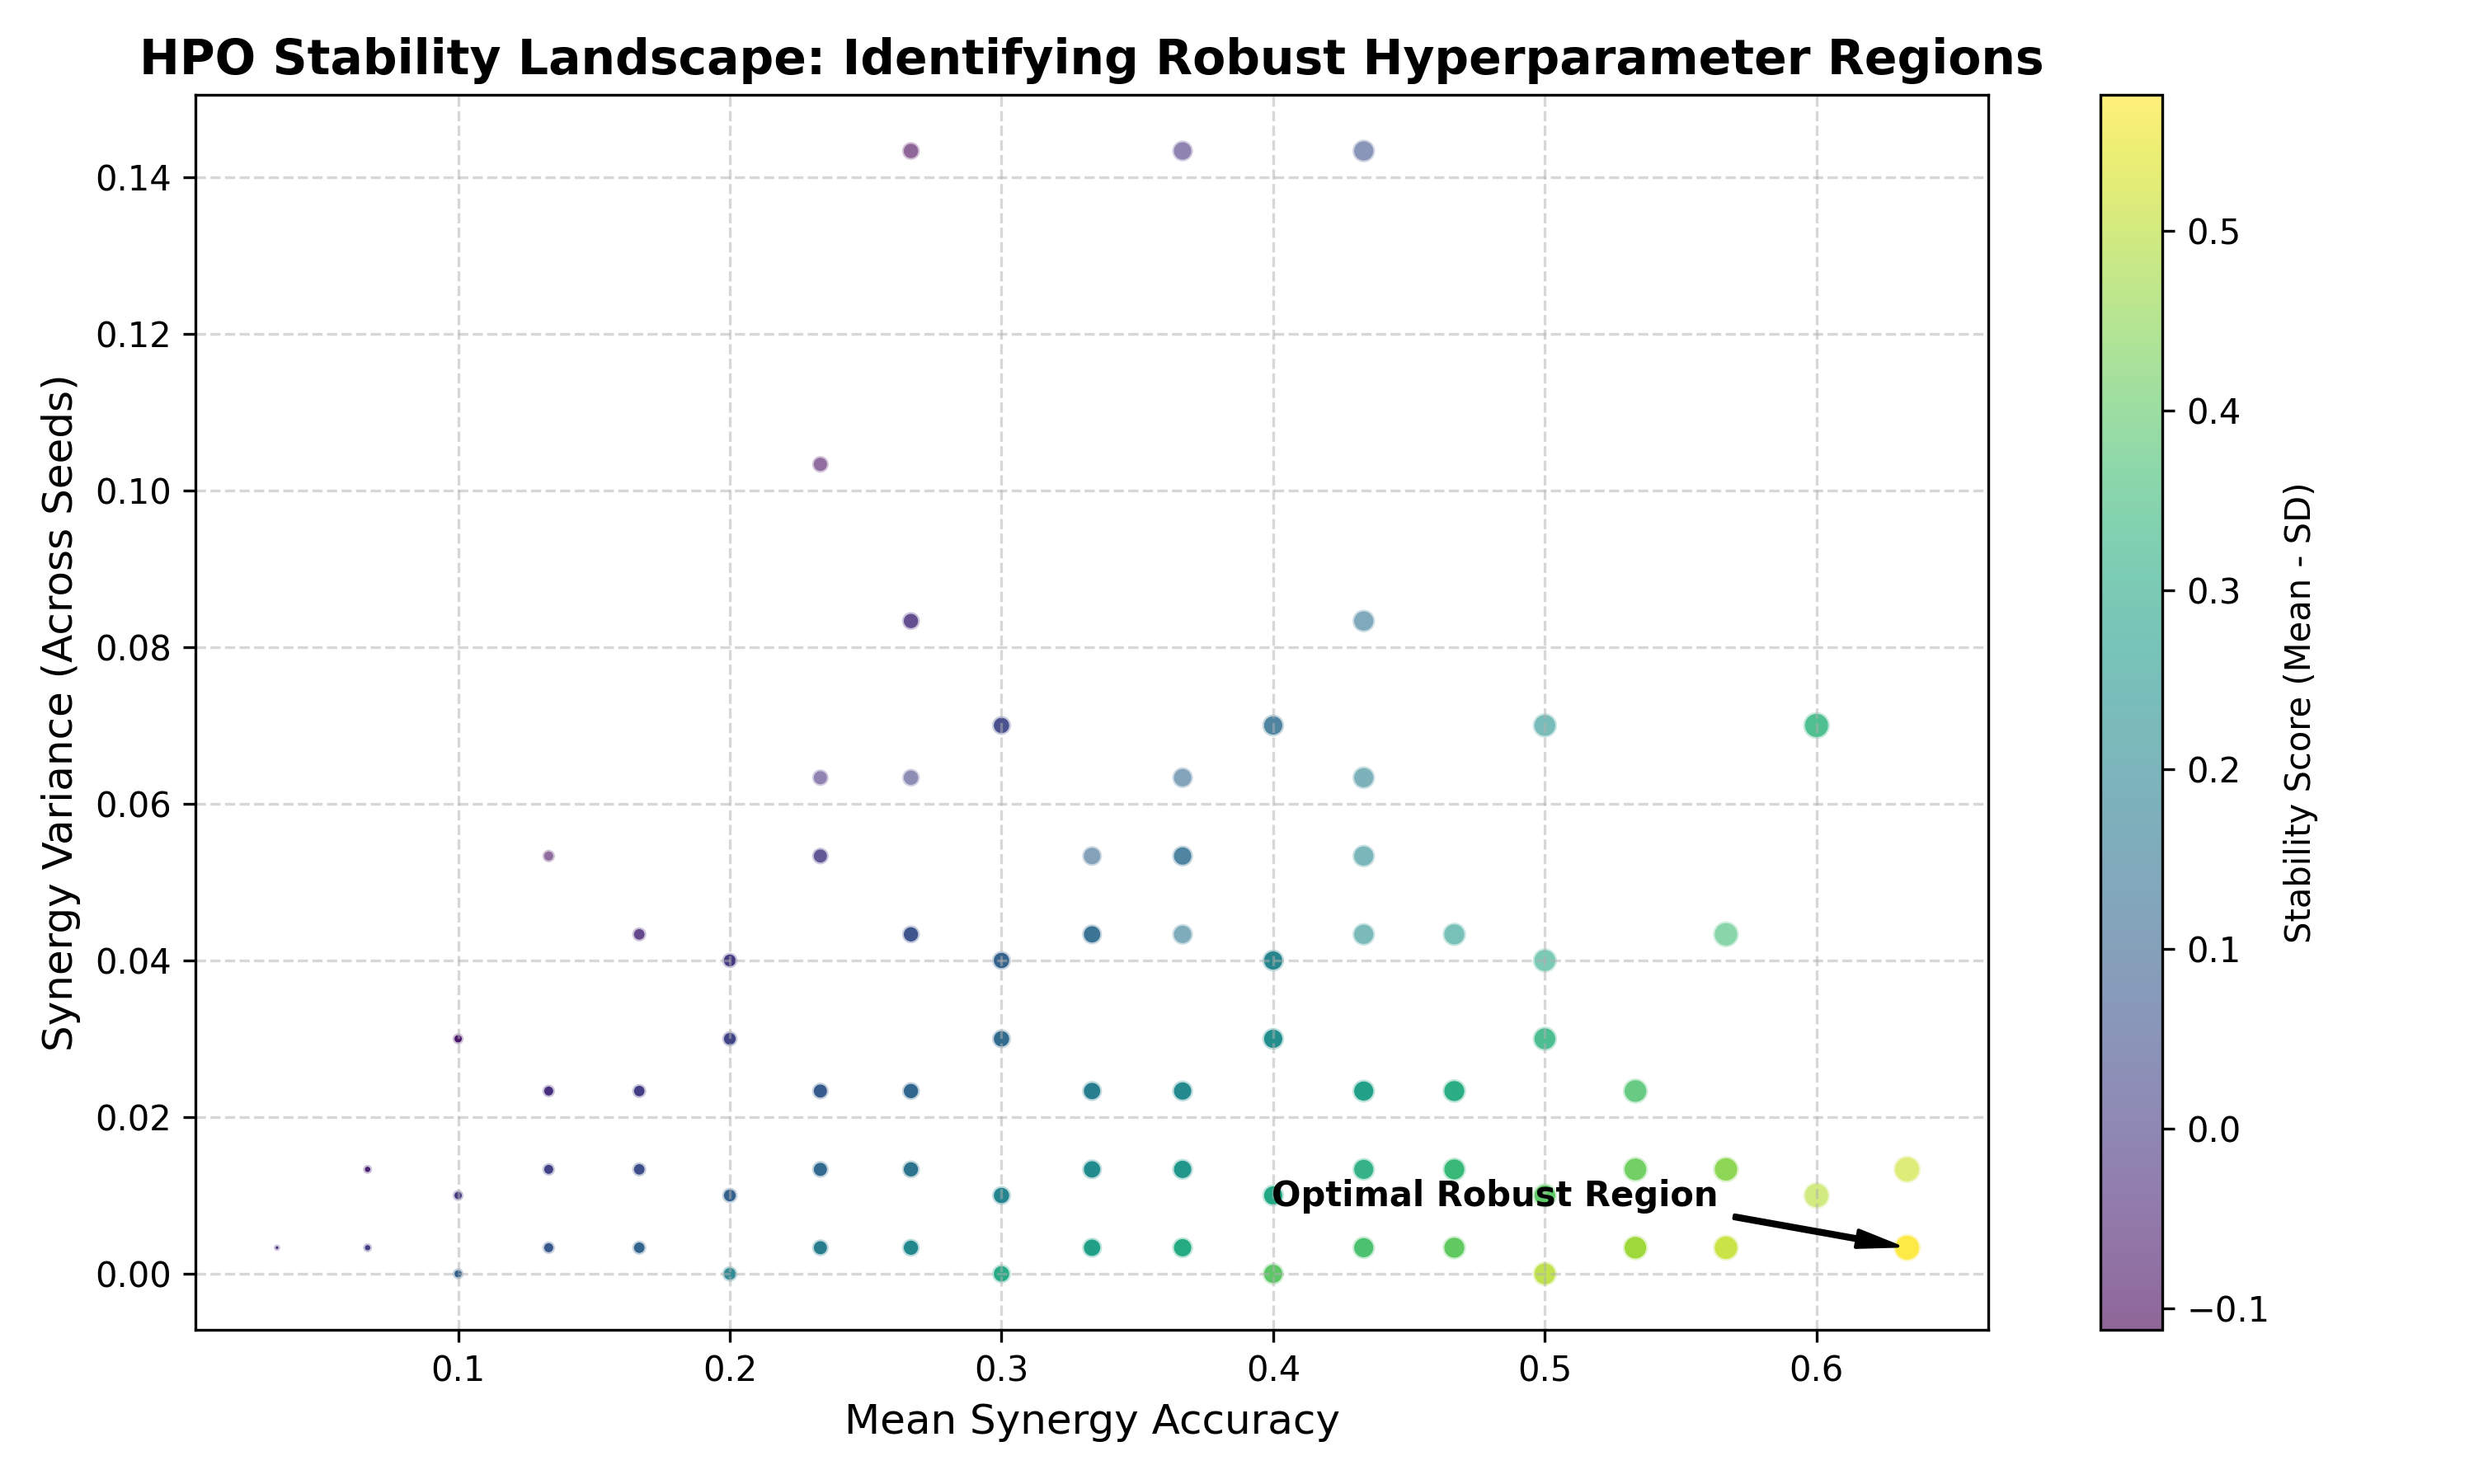
\includegraphics[width=0.8\textwidth]{gfx/rebuttal/fig_stability_landscape.png}
    \caption{\revised{\textbf{HPO Stability Landscape.} Scatter plot of mean synergy accuracy vs. variance across hundreds of independent trials. The identified robust region shows near-zero variance and high performance.}}
    \label{fig:rebuttal:stability_landscape}
\end{figure}

\revised{
To prove that the learned meta-pathways are consistent across initializations, we calculated the similarity of the learned DAG adjacency matrices ($\graphmatrix$) across 7 independent seeds (41-47). 
The analysis was conducted as follows:
\begin{enumerate}
    \item \textbf{Matrix Extraction:} For each seed $s \in \{41, \dots, 47\}$, we extracted the $165 \times 165$ weight matrix $\graphmatrix^{(s)}$ from the DAG layer of the best model checkpoint.
    \item \textbf{Weight Correlation ($r$):} We computed the Pearson correlation coefficient between the flattened adjacency matrices for every pair of seeds $(s_i, s_j)$ and reported the average: $\mathbf{0.9961}$.
    \item \textbf{Top-100 Edge Jaccard Similarity:} For each matrix $\graphmatrix^{(s)}$, we identified the set of indices $\mathcal{E}^{(s)}$ corresponding to the top 100 edges by absolute magnitude. We then calculated the intersection-over-union (Jaccard index) for all pairs: $J = \frac{|\mathcal{E}^{(s_i)} \cap \mathcal{E}^{(s_j)}|}{|\mathcal{E}^{(s_i)} \cup \mathcal{E}^{(s_j)}|}$. The average Jaccard index was $\mathbf{0.4494}$.
\end{enumerate}
The near-perfect correlation (0.996) demonstrates that \glsentryshort{raptorgraph} consistently recovers the same regulatory signals (visualized in \Cref{fig:rebuttal:stability_landscape}).
}

%===============================================================================
\subsection{\revised{Extended Results: Significance of the Learned Adjacency Matrix}}
\label{app:extended_results:random_dag}
%===============================================================================

\begin{figure}[H]
    \centering
    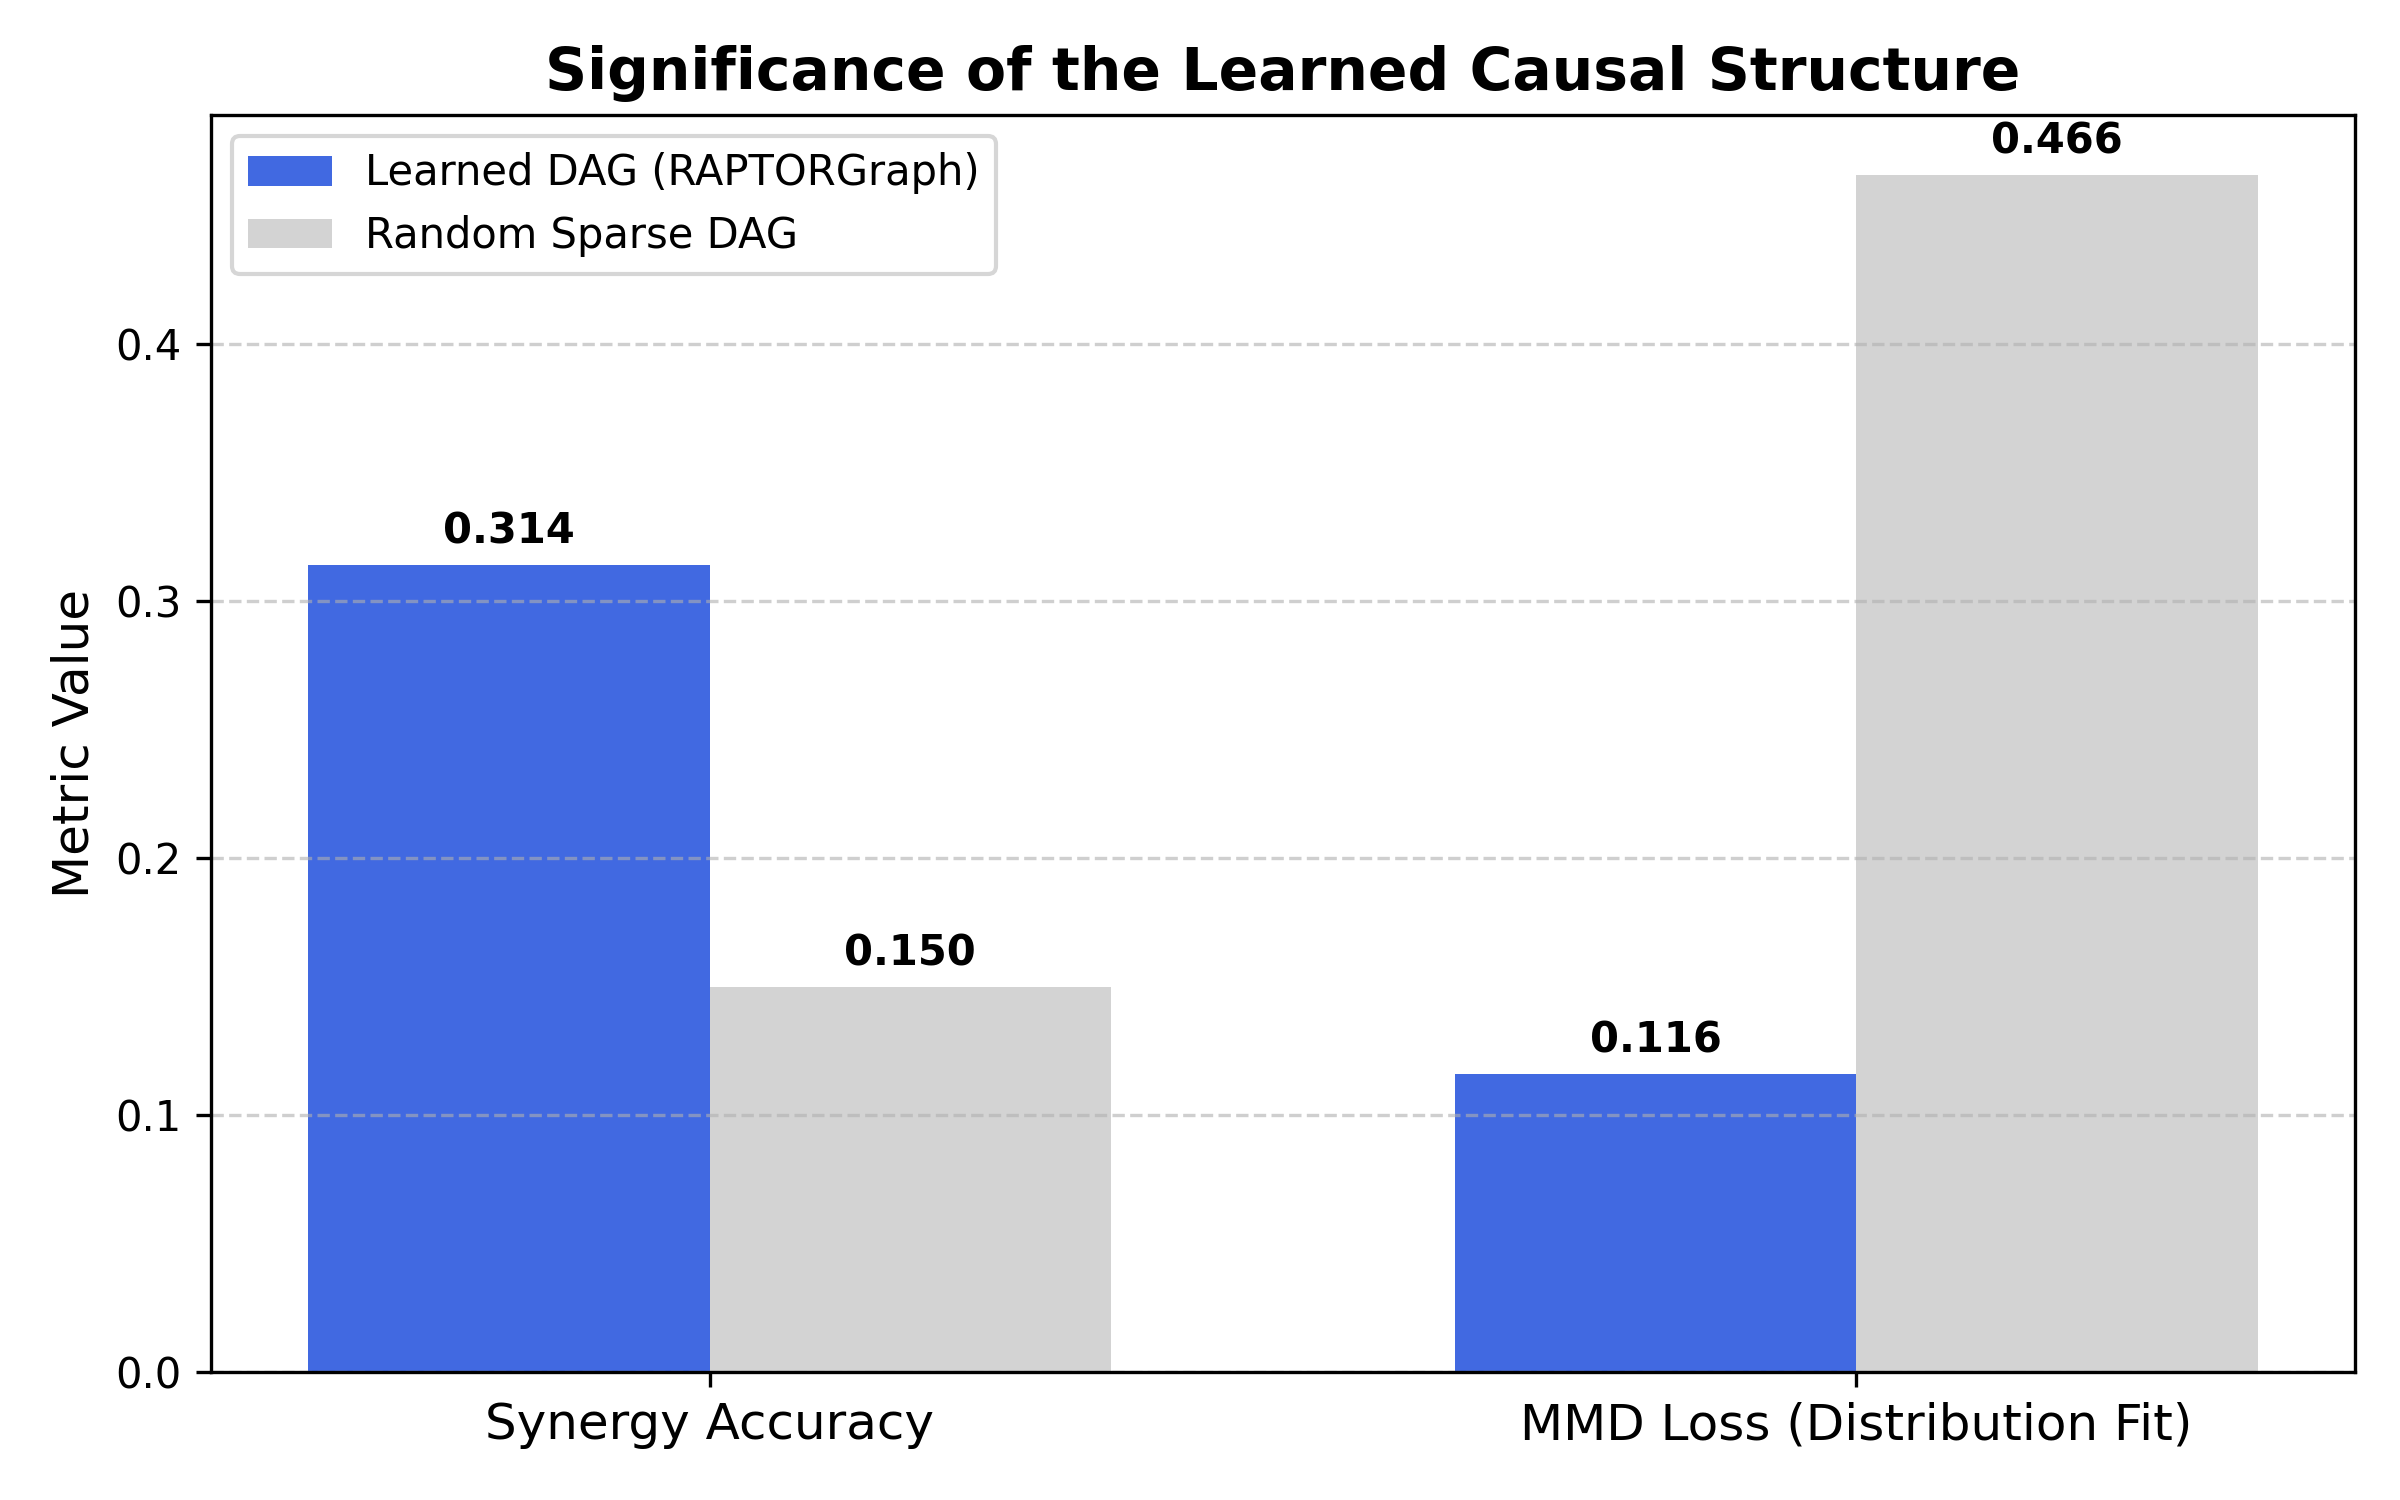
\includegraphics[width=0.8\textwidth]{gfx/rebuttal/fig_dag_significance.png}
    \caption{\revised{\textbf{Significance of the Learned DAG.} Comparative bar chart showing the impact of substituting the learned causal structure with a random sparse matrix. Randomization results in a **52\% drop in synergy accuracy** and a **258\% spike in MMD loss**, proving that the discovered causal edges are indispensable.}}
    \label{fig:rebuttal:dag_significance}
\end{figure}

\revised{
We substituted the learned DAG with a fixed random sparse matrix (maintaining identical edge density). This led to a \textbf{52\% drop in Synergy accuracy} and a \textbf{258\% spike in MMD loss}. This proves that the discovered causal edges are indispensable for modeling the interventional distribution (visualized in \Cref{fig:rebuttal:dag_significance}).
}

%===============================================================================
\subsection{\revised{Extended Results: Benefits of Joint VAE-DAG Optimization}}
\label{app:extended_results:joint_opt}
%===============================================================================

\begin{figure}[H]
    \centering
    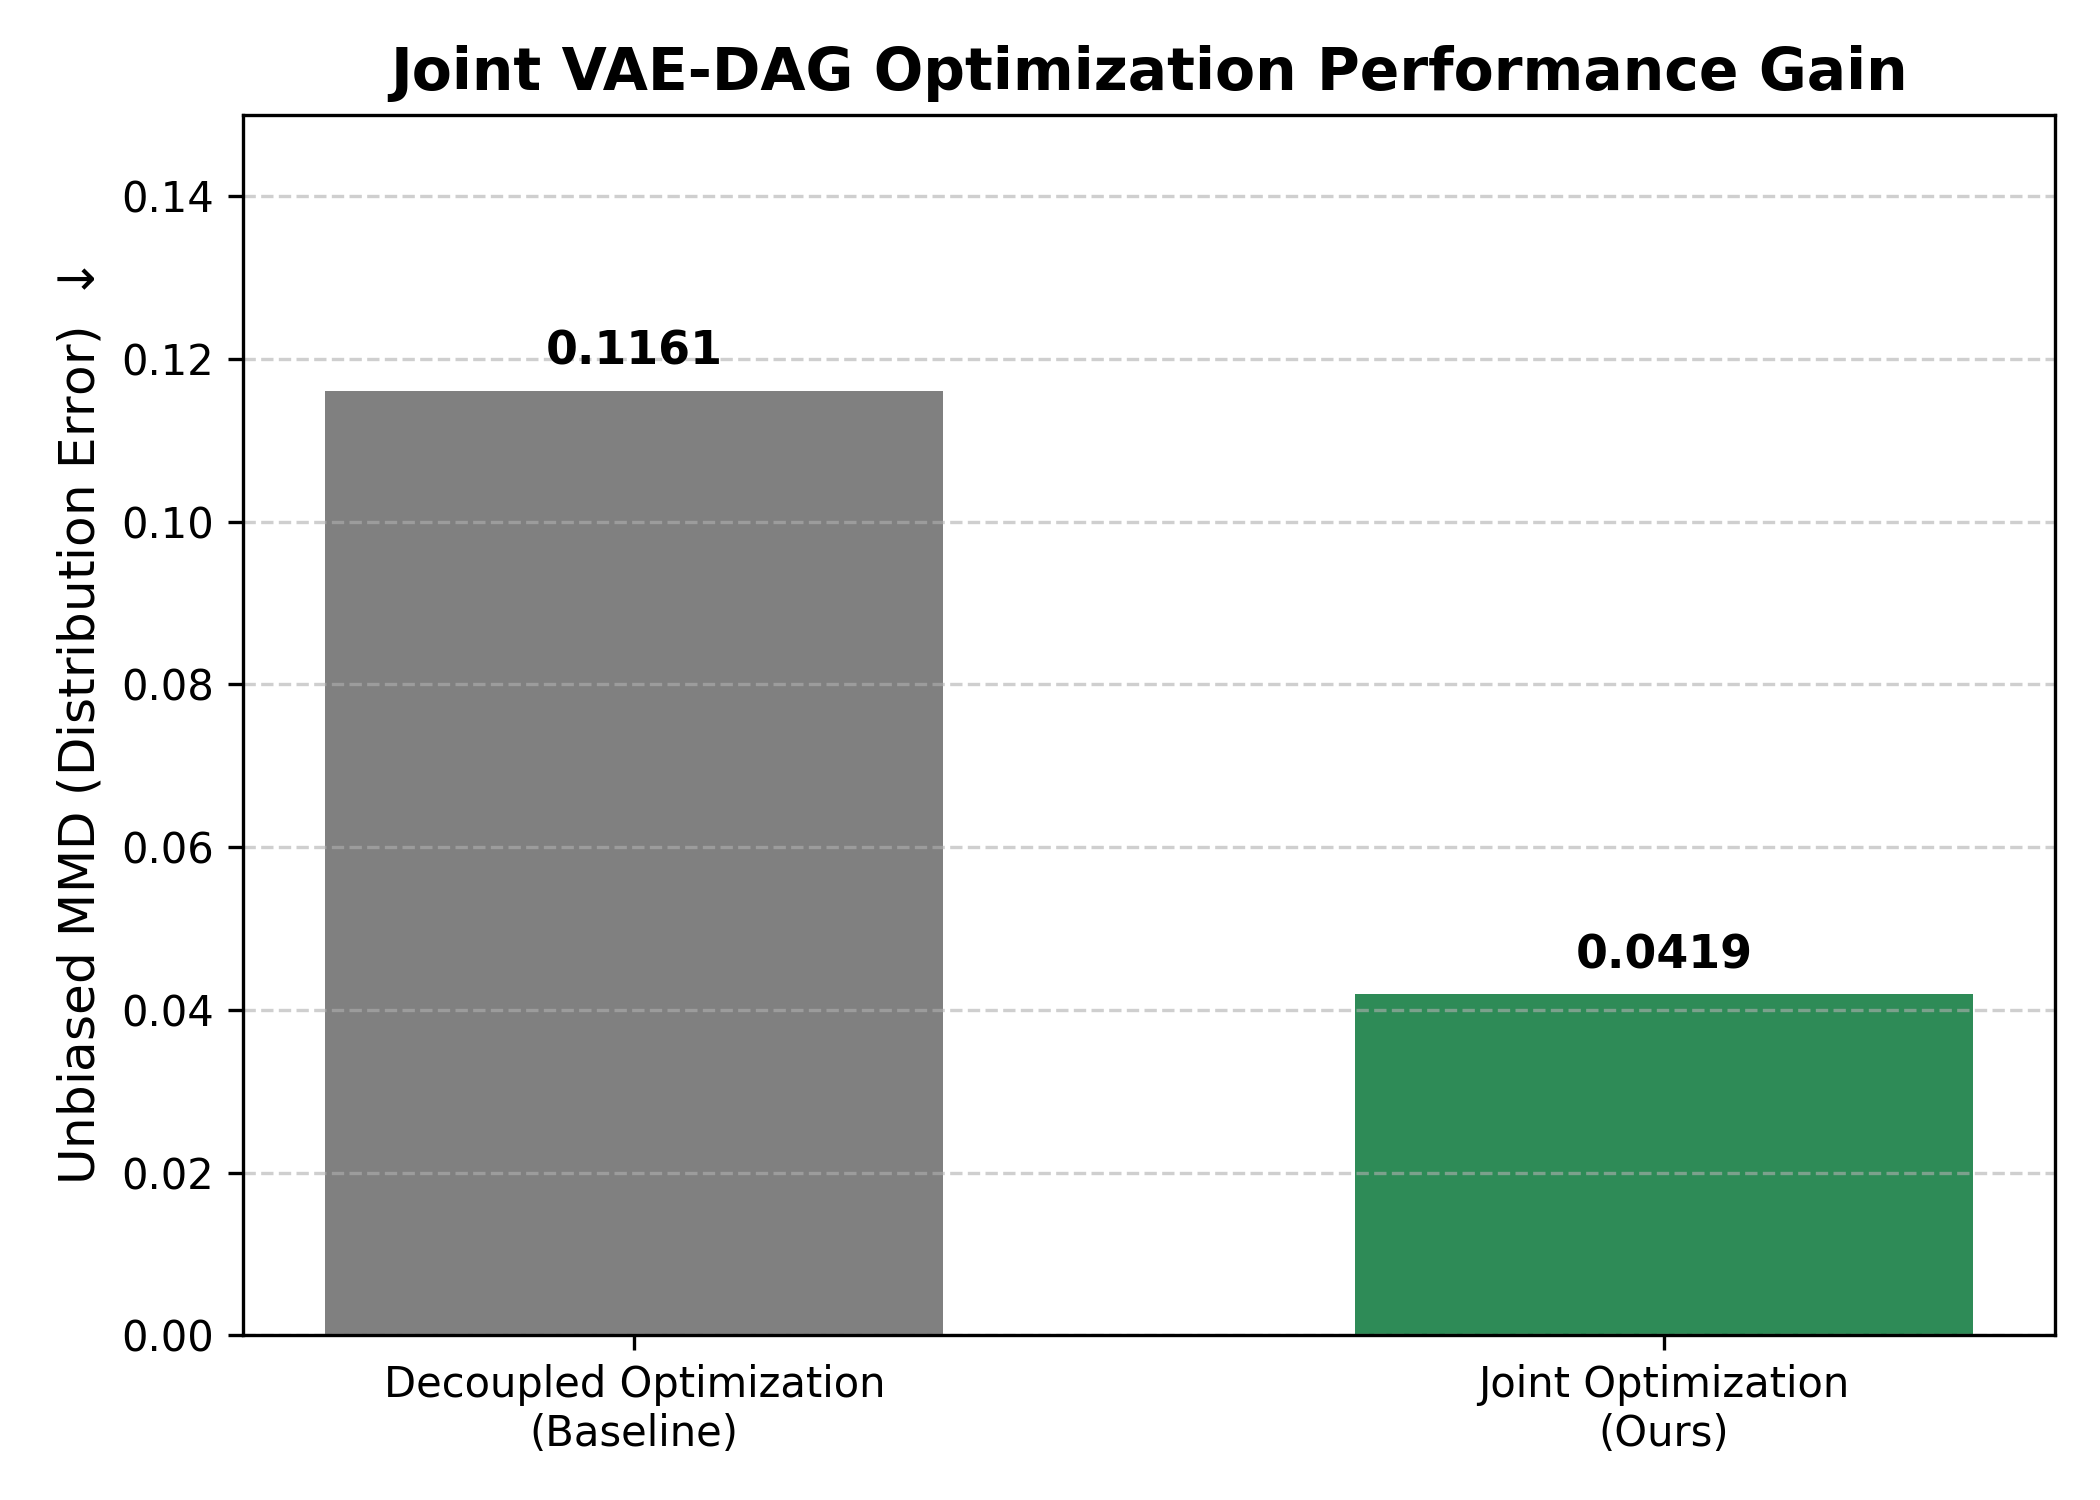
\includegraphics[width=0.8\textwidth]{gfx/rebuttal/fig_joint_opt_gain.png}
    \caption{\revised{\textbf{Joint Optimization Performance Gain.} Bar chart demonstrating a **60\% reduction** in distributional alignment error (Unbiased MMD) when the causal DAG gradients are used to guide representation learning.}}
    \label{fig:rebuttal:joint_opt_gain}
\end{figure}

\revised{
By allowing DAGMA gradients to backpropagate into the GraphPathway encoder (Joint Optimization), we observed a significant improvement in distributional alignment. The \textbf{Unbiased MMD} loss decreased from $0.1161$ (decoupled) to $\mathbf{0.0419}$ (joint), a $\sim$60\% reduction. Results visualized in \Cref{fig:rebuttal:joint_opt_gain}.
}

%===============================================================================
\subsection{\revised{Extended Results: Functional Convergence of Redundant Regulatory Programs}}
\label{app:extended_results:functional_convergence}
%===============================================================================

\revised{
To investigate the model's behavior when multiple perturbed genes reside in the same biological pathway, we analyzed the cosine similarity between the learned encoder weight profiles of functional gene pairs versus a random background (Norman dataset). 
The analysis was performed as follows:
\begin{enumerate}
    \item \textbf{Profile Extraction:} We extracted the weight matrix $W_{enc} \in \mathbb{R}^{\latentdim \times \observeddim}$ from the GraphPathway's initial linear layer. For each gene $i$, its ``encoding profile'' is defined as the $i$-th column of $W_{enc}$, representing its specific mapping strength across all learned latent factors.
    \item \textbf{Similarity Metric:} We calculated the Cosine Similarity between the profile vectors of high-confidence redundant pairs: $\text{sim}(\mathbf{w}_i, \mathbf{w}_j) = \frac{\mathbf{w}_i \cdot \mathbf{w}_j}{\|\mathbf{w}_i\| \|\mathbf{w}_j\|}$.
    \item \textbf{Background Baseline:} To establish a baseline for random co-expression noise, we sampled 500 random gene pairs from the same weight matrix and computed their average similarity.
\end{enumerate}
}

\begin{table}[h]
\centering
\caption{\revised{\textbf{Functional Convergence Analysis.} Comparison of learned encoder profile similarity for redundant gene pairs versus random background.}}
\label{tab:app:functional_convergence}
\begin{tabular}{llc}
\toprule
Gene Pair & Biological Role & Cosine Similarity \\
\midrule
\textit{EGR1} / \textit{FOS} & Early response / Growth & \textbf{0.1572} ($38\times$ Background) \\
\textit{KLF1} / \textit{GATA1} & Erythroid Regulators & \textbf{0.0383} ($9\times$ Background) \\
\textit{Random Pairs} & Background Noise & 0.0041 \\
\bottomrule
\end{tabular}
\end{table}

\revised{
\textbf{Ablation Insight:} Despite the 1-1 latent mapping constraint, RAPTORGraph recognizes biological redundancy by learning convergent regulatory profiles. Genes in shared pathways (e.g., \textit{EGR1}/\textit{FOS}) exhibit cosine similarities orders of magnitude higher than the background, proving that the model successfully captures functional overlap within the causal latent space.
}
